
\documentclass[numbers=noenddot, abstract=on, a4paper, headsepline,
footsepline, oneside, draft=off]{scrreprt}

% Setting heading fonts to serif
\addtokomafont{disposition}{\rmfamily}

% Setting description label fonts to serif
\addtokomafont{descriptionlabel}{\rmfamily}

\usepackage[T1]{fontenc}


\usepackage[english]{babel} 
\usepackage[utf8]{inputenc}

% biblatex
\usepackage[backend=bibtex8]{biblatex}
\bibliography{bib/bibliography.bib}

% switch last names in bibliography to small caps
\renewcommand*{\mkbibnamelast}[1]{\textsc{#1}}

% we need these packages for the gantt chart
\usepackage{pgfgantt}
\usepackage{rotating}

% We need this to display the group symbols correctly
\usepackage{amssymb}
\usepackage{amsmath}

\usepackage{upgreek}

% activate the headings
\pagestyle{headings}
% make sure that the headings also appear on the first page of the chapter
\renewcommand*{\chapterpagestyle}{headings}
% change the font of the headings to smallcaps
\setkomafont{pagehead}{\scshape}

% UML stuff
\usepackage{tikz}
\usepackage{tikz-uml}

\usetikzlibrary{matrix, arrows}

% Intelligent references
\usepackage{varioref} 

% Nomenclauture
\usepackage{nomencl}

% Draft watermark
\usepackage[firstpage]{draftwatermark}
\SetWatermarkScale{5}
\SetWatermarkLightness{0.9}



% improve word spacing
\usepackage{microtype}

% Using links in PDFs, but without the ugly borders
\usepackage{hyperref}
\hypersetup{
    colorlinks=false,
    pdfborder={0 0 0},
    pdfauthor={Juerg Ritter},
    pdftitle={Decentralized E-Voting on Android Devices Using Homomorphic
    Tallying},
    pdfsubject={Master Thesis},
    pdfkeywords={E-Voting;Android;Master Thesis},
}

\usepackage{cleveref}


% definitions of own commands
%\newcommand{\myref}[1]{(see section \ref{#1} on page \pageref{#1})}
\newcommand{\myref}[1]{(see \Vref{#1})}

\usepackage[enabled]{easy-todo}

% Pretty tables
\usepackage{tabularx}
\usepackage{booktabs}

\begin{document}

\title{\bf Decentralized E-Voting on Android Devices Using Homomorphic Tallying}
\subject{Master Thesis}
\author{Juerg Ritter (\url{rittj1@bfh.ch})\\
\\
Bern University of Applied Sciences\\
Engineering and Information Technology\\
CH-2501 Biel, Switzerland\\
}
\date{\today}
\publishers{Advisor:\\
Prof. Dr. Rolf Haenni, Bern University of Applied Sciences\\
\bigskip
Expert:\\
Stephan Neumann, Technical University of Darmstadt}
\maketitle

\makenomenclature

\clearpage
\pagenumbering{roman}

\begin{abstract}
The E-Voting Group of the Bern University of Applied Sciences is planning to
evaluate decentralized e-voting systems for practical use. The term
``decentralized'' in that context means that there is no central server
infrastructure involved in the voting process. The main application of such
e-voting systems are votes with a low number of participants, for example the
board of directors in a company. The idea is, that the participants create an
ad-hoc network with mobile devices. The main goal of this master thesis is to
implement a decentralized e-voting system for Android based mobile devices. We
are using a voting scheme that uses homomorphic tallying and secret sharing to
guarantee privacy and verifiability. It also provides robustness in the sense
that it is not possible for a single party to break the voting process just by
refusing the collaboration at a certain step throughout the voting process. A
big focus area is also the usability of this system, it should be possible for
participants without extensive knowledge in the area of information security to
use this e-voting system.
\end{abstract}

\tableofcontents
\listoffigures
\listoftables

% Nomenclature 
% ------------------------------------------------------------------
\nomenclature{$p, q, g$}{The ElGamal parameters}
\nomenclature{$m$}{A cleartext message}
\nomenclature{$(a, b)$}{An ElGamal ciphertext tuple}
\nomenclature{$x$}{An ElGamal private key}
\nomenclature{$y$}{An ElGamal public key}


\printnomenclature
% ------------------------------------------------------------------

\chapter{Introduction}
\pagenumbering{arabic}
\label{cha:introduction}
The history of voting on a particular question in order determine the will of a
group of people goes far back to the ancient Greeks, who laid the groundwork of
today's democratic societies. Over the years, the purpose of holding elections
remained the same, while the procedures on how voting is done has changed
significantly. The most ancient way of expressing the will by a hand sign has
been replaced by modern technologies. The 20th century has seen a lot of changes
in this area. Paper based voting has been introduced, and with the
industrialization, the first voting machines appeared on the surface. The
purpose of these machines was to simplify the counting process. In today's internet
society where a lot of tasks such as banking, shopping, mailing, etc. has been
revolutionized by the internet, it is not surprising that there are a lot of
efforts going on to revolutionize the process of voting as well.

One of the research fields of the Bern University of Applied Sciences is the
area of e-voting. E-voting has become a big field of research in the past couple
years. Still, there is no generic approach which meets all the criteria such as
privacy, transparency, etc. which we want in e-voting. These properties are
discussed in \Vref{sec:evoting}. The e-voting research group of the Bern
University of Applied Sciences \cite{www:EVG} tries to improve this situation with the following approaches:
\begin{itemize}
  \item Develop new approaches and provide them to the community for review.
  \item Take existing approaches and evaluate them in terms of practicability.
  These approaches are usually available as scientific papers.
\end{itemize}

The evaluation of these approaches is usually done by implementing them into a
prototype level application. This implementation is used to show that the
approach works in practice and provides a certain usability. The E-Voting Group
would like to gain some experience on how decentralized e-voting systems could
be implemented and how they behave in practice. There are some approaches which
focus explicitly on decentralized e-voting systems, such as the proposal of
Dalia Khader et al. \cite{HKRS12}. In this project however, we would like to adapt the
voting scheme proposed by Cramer et. al. \cite{CGS97} in a way that it can be
used as a decentralized e-voting system.

A possible use case of such a system could be an executive board or any other
commitee that would like to vote on some matters without having their members
to reveal what exactly they voted for. The architecture of our system requires
that all the participants are in a confined space and are able to exchange some
sort of credential using a communication channel which relies on physical
proximity (e.g. near field communication) or visual contact (e.g. QR-codes).

In previous projects during the master studies, some groundwork has been
implemented which can now be used as a foundation for this project. The
previously implemented projects are the following:
\begin{itemize}
  \item \textbf{UniCrypt:} UniCrypt is a cryptographic library developed by the
  members of the E-Voting Group of the Bern University of Applied Sciences. It
  provides cryptographic building blocks such as the ElGamal cryptosystem, zero
  knowledge proofs, digital signatures, etc. 
  \item \textbf{InstaCircle: } InstaCircle provides a decentralized
  communication platform for Android devices. It allows to exchange messages
  using Wi-Fi communication among a closed user group.
\end{itemize}
The projects mentioned above will be discussed in more detail in \Vref{cha:brw}.

\section{Goals}
\label{cha:goals}
The final result of this project is a fully-fledged decentralized e-voting
application which runs on Android devices and does not require any equipment
other than the Android smartphones or tablets. The CGS97 e-voting
scheme \cite{CGS97} will be used as the theoretical foundation for this project.
Having said this, we divide the following goals for this project:
\paragraph{E-Voting Functionality.}
The main goal of this project is the implementation of the logic of CGS97
\cite{CGS97}, by assembling the cryptographic building blocks to a working
application. It has to be tied to the user interface and to InstaCircle for
communicating with the other participants. This part is heavily based on already
existing components, namely InstaCircle which provides the decentralized
communication infrastructure and UniCrypt which provides the implementation of
the cryptographic building blocks which are used in CGS97
\myref{sec:buildingblocks}. The final product needs to be able to handle a
voting scenario \emph{one-out-of-n}, meaning that a user can choose exactly one
out of $n$ options. This allows to set up votes which are more complex
than a simple \emph{Yes-No} vote. At the other end of the spectrum would be the
\emph{m-out-of-n} scenario, that means that $m$ options can be picked out of $n$
options. The \emph{m-out-of-n} scenario is not a must for this project.

\paragraph{Extension of UniCrypt.}
UniCrypt implements many cryptographic building blocks which are necessary in
order to implement a CGS97 based e-voting system, however two crucial parts are
missing:
\begin{itemize}
  \item \textbf{ElGamal Proof of Validity:} This type of zero-knowledge proof is
  used in order to make sure that a ciphertext is an ElGamal encryption of an
  element which belongs to a set of possible plaintexts. This type of proof is
  an instance of of a more generic \emph{OR-composition} of multiple proofs of
  knowledge. This type of zero-knowledge proof is discussed in detail in
  \Vref{sec:zeroknowledgeproofs}.
  \item \textbf{Threshold Cryptosystem:} In order to ensure privacy of
  the ballots, the CGS97 e-voting scheme uses a so called threshold system. This
  system allows to split a secret key and distribute \emph{key shares} to a
  given set of participants. In order to decrypt a ciphertext, the parties have
  to collaborate in order to reconstruct the secret key. Threshold cryptosystems
  are discussed in further detail in \Vref{sec:secretsharing}.
\end{itemize}

As a goal of this project, these two essential building blocks have to be
implemented and integrated into the UniCrypt library.

\paragraph{Graphical User Interface.}
In many cases, cryptographic functions which are heavily used in the context of
e-voting have a negative impact on the usability. Many steps such as key
generation, decryption, etc. have to be done in order to guarantee all the
desired properties for e-voting. All these steps bring a certain complexity
into the handling of the application. Therefore it is crucial to guide the user
through the process, and this can only be done by providing them a carefully
crafted user interface. A further goal of this project is to implement a user
interface which provides a good usability.
\\

The time budget of this master thesis is one year, although the project will be
implemented part time. It is equivalent to 27 ECTS credits.

\section{Contribution}
\label{sec:contribution}
Currently there are a couple of Android apps available in the Google Play store
\cite{www:playstore} which allow to do simple votes, or else they are clients of e-voting
systems of a specific organisation. A decentralized e-voting system which offers the
cryptographic level of this project is currently not available. The
implementation and the evaluation of this project will help to understand
further strong and weak points of the CGS97 e-voting scheme, especially when
using it in a decentralized configuration. So far, the E-Voting Group of the
Bern University of Applied Sciences has gained expertise by implementing and
operating e-voting systems on centralized systems which are usually operated on
notebooks or desktop computers. This project will help gaining some experience
in how e-voting systems can be used on mobile devices.

Furthermore, the extensions for the UniCrypt library can be used for other
projects as well. In the area of e-voting, threshold cryptosystems and validity
proofs are considered as standard building blocks and can be used for the
implementation of e-voting schemes other than CGS97.

\section{Outline}
\Vref{cha:brw} gives an overview of the work on which this project has
been based on. The cryptographic building blocks which are used are discussed,
as well as the e-voting scheme on which this work is based on. We also discuss
projects which have been implemented as a preparation of this master thesis.
\Vref{cha:results} explains the resulting implementation in detail.

\todo{Needs to be extended with results, discussion and conclusion}

\chapter{Background and Related Work}
\label{cha:brw}
This section gives an overview of the theoretical foundations and some projects
which have been implemented earlier in order to serve as a foundation for this
project. 

\section{E-Voting in 2013}
\label{sec:evoting}
In today's internet world, many tasks such as sending mail, doing bank
transactions, booking flights etc. can be done using the internet. Instead of
going to the post office, to the bank or the travel agency, one can complete
these tasks in a very comfortable fashion at home in front of the computer. Not
surprisingly, people have thought about replace the way to the voting station
with an internet based solution. This so called e-voting has appeared on the
surface soon after the quick rise of the internet, but so far the big
breakthrough has not happened, which might be surprising at first sight.
Instead, the area of e-voting has become a big research area, tightly related to
the area of cryptography.

Let us have a closer look at the reasons why e-voting
could not find it's way to success so far. For a better understanding, we should
identify the properties that we expect from an e-voting system. Over the time,
some properties and their definitions have emerged.

\begin{description}
  \item[Democracy:] Only eligible voters can vote, and each voter can
  cast at most one ballot which will be included in the result.
  \item[Accuracy:] The result is derived from \emph{all} valid
  votes as they were cast, i.e. cast votes can not be modified. No other factors
  than valid votes can influence the result.
  \item[Universal verifiability:] Anyone can verify the correctness of
  the result.
  \item[Individual verifiability:] A voter can can verify that her vote
  is included in the result as she cast it.
  \item[Privacy:] Nobody can obtain information how a voter has
  voted.
  \item[Receipt-freeness:] The voter can not prove to anybody else how
  she voted.
  \item[Coercion-resistance:] Noone can force a voter to vote in a
  particular way, or prevent a voter to vote at all.
  \item[Robustness:] An attacker is not able to disrupt an election
  process or change the outcome by damaging a small set of system components. 
\end{description}

All these properties are discussed in detail in \cite{HS11} and \cite{Jonker09}.
As it turns out, it is not at all easy to build a system that meets all these
desired requirements. Not even the classic paper based voting meets all the
requirements, for example the verifiability is not given in a classic voting
scenario. Researchers are trying to develop schemes towards these requirements
using cryptographic building blocks. The robustness property is probably the
biggest factor that prevents the breakthrough of e-voting on large scales.
E-voting systems are the perfect targets for an intended manipulation or a
boycott of an election. That's why many governments use e-voting only on small
scales so that the electorate is small enough that it is statistically unlikely
to tip the scale to one side or the other.

\section{Cryptographic Building Blocks}
\label{sec:buildingblocks}
The voting scheme that will be used in our system is assembled from some well
known cryptographic building blocks which are briefly explained in this section.
All these cryptographic building blocks belong to the area of \emph{asymmetric}
cryptography, which is based usually based on key pair, containing a
\emph{public key} and a \emph{secret key}.

\subsection{Discrete Logarithm Problem}
Asymmetric cryptography relies on a mathematical problem, which is nowadays
considered to be hard to solve, meaning that so far there is no known algorithm
to find a solution for a given problem efficiently. An example of such a problem
is the prime factorization of large numbers on which the security of the famous
RSA cryptosystem \cite{RSA78} is based on. The other hard problem of this kind
is know as the \emph{Discrete Logarithm Problem}. The formal definition of
the problem is as follows: 

Given a prime $p$, a generator $g$ of a multiplicative modular group
$\mathbb{Z}^*_p$ and an element $b \in \mathbb{Z}^*_p$, find the integer
$x,0 \leq x \leq p - 2$, such that $a^x \equiv b \mod p$.

Currently there is no efficient way of solving this equation in an efficient
manner. There are some more sophisticated approaches than the naive way of
iterating over all elements of the group, for example the baby-step giant-step
algorithm. The security of most of the building blocks we are using in this
project is based on this problem. Further information concerning the discrete
logarithm problem can be found in Chapter 3 of the Handbook of Applied
Cryptography by Alfred Menezes et. al. \cite{book:hac}.

\subsection{ElGamal Cryptosystem}
\label{sec:elgamal}
The ElGamal cryptosystem \cite{EG84}, proposed by Taher El Gamal in 1984, is the
asymmetric cryptosystem which is mostly used in the context of e-voting. An
asymmetric cryptosystem uses two keys to operate, one which is used to encrypt a
certain message (the public key) and another to decrypt the message (the secret
key). The security of this cryptosystem is based on the fact that it is hard to
compute the logarithm in discrete modular groups and hence making the
exponentiation in modular groups a one way function. A major advantage of the
ElGamal cryptosystem is the fact, that the encryption function includes a random
value. Especially in the context of e-voting this is a crucial property, because
when encrypting a value (for example the value $1$ which means \textit{Yes}),
the resulting ciphertext is always different. That is why ElGamal is also called
a \textit{randomized} cryptosystem.

In order to define an ElGamal cryptosystem, three parameters are required. Let
$p$ and $q$ be large prime numbers such that $q|p-1$.\footnote{In the case of
$p=2q+1$ where $p$ and $q$ are primes, $p$ is called \emph{save prime} and $q$
is called \emph{Sophie Germain prime}.}
The prime number $q$ defines the order of a subgroup $G_q$ of the multiplicative
modular group $\mathbb{Z}^*_p$. $\mathbb{Z}_q$ is an additive modular group of order $q$. The
last parameter needed is an arbitrarily chosen generator $g$ of the group $G_q$.
Further information concerning group theory can be found in Chapter 2 of the
Handbook of Applied Cryptography by Alfred Menezes et. al. \cite{book:hac}. We
can now derive the asymmetric key pair containing the secret key $x \in_R
\mathbb{Z}_q$ and the public key $y=g^x \in G_q$. A message $m \in G_q$ can be
encrypted by first choosing a random value $r \in_R \mathbb{Z}_q$, and then
applying the following function:
\begin{equation}
Enc_y : G_q \times \mathbb{Z}_q \rightarrow G_q \times G_q,
(a, b)=Enc_y(m, r)=(g^r, y^r \cdot m) \notag
\end{equation}
The tuple $(a, b)$ is the ciphertext of the message $m$. $m$ can be recovered using the secret key $x$
by applying the decryption function:
\begin{equation}
Dec_x : G_q \times G_q \rightarrow G_q,
m=Dec_x(a, b)=a^{-x} \cdot b \notag
\end{equation}

\subsubsection{Exponential ElGamal}
\label{sec:expelgamal}
In the area of e-voting, we often find a slight variation of ElGamal which is
called \emph{exponential ElGamal}. In exponential ElGamal, we encode a message
$\hat{m}$ by using a generator $\hat{g}$ of $G_q$ and raise it to the power of
the message $\hat{m} \in \mathbb{Z}_q$. In many cases, the ElGamal parameter $g$
is used as $\hat{g}$, which makes it unnecessary to define a fourth predefined
parameter. Note that the message $\hat{m}$ is an element of the additive group
$\mathbb{Z}_q$ as opposed to the classical ElGamal where $m$ is an element of
the multiplicative group $G_q$. Elements of the group $\mathbb{Z}_q$ are much
easier to find as all integers between $0$ and $q-1$ belong to this group. The
modified encryption function of exponential ElGamal looks as follows:
\begin{equation}
\hat{Enc_y} : \mathbb{Z}_q \times \mathbb{Z}_q \rightarrow G_q \times G_q,
(a, b)=\hat{Enc_y}(\hat{m}, r)=(g^r, y^r \cdot \hat{g}^{\hat{m}}) \notag
\end{equation}
In order to decrypt a given ciphertext, we apply the ordinary ElGamal decryption
function and obtain the value $\hat{g}^{\hat{m}} \in G_q$. To reveal $\hat{m}$,
we would have to compute the discrete logarithm, which is a hard problem in
general. If we have knowledge about all the possible plaintexts (e.g. we know
that a ballot either contains 0 for \emph{no} or 1 for \emph{yes}), we can just try all
possible plaintexts. 

Exponential ElGamal has another property which is important in the context of
e-voting: It transforms the right part of the ElGamal encryption function from a
multiplicative homomorph function into an additive homomorph function.
Homomorphic encryption is discussed in detail in \Cref{sec:homenc}.

\subsection{Homomorphic encryption}
\label{sec:homenc}
The ElGamal cryptosystem has a property
which is important for building verifiable e-voting schemes, namely the property
of \emph{homomorphism}. Given two mathematical groups $(X,\oplus)$ and
$(Y,\otimes)$, a mathematical function $f:X \rightarrow Y$ is $(\oplus, \otimes)$-homomorphic if
the following condition holds:
\begin{equation}
f(m_1) \otimes f(m_2) = f(m_1 \oplus m_2) \notag
\end{equation}
The ElGamal function offers exactly that property for its encryption function
$Enc_y:G_q \times \mathbb{Z}_q \rightarrow G_q \times G_q$ using the same public key $y$:
\begin{equation}
Enc_y(m_1, r_1) \cdot Enc_y(m_2, r_2) = Enc_y(m_1 \cdot m_2, r_1 + r_2)
\notag
\end{equation}
This property allows to calculate the encrypted product of all messages out of
the encrypted messages and decrypt only the result. Applied to e-voting, the
result can be computed out of the encrypted ballots and only the final result
needs to be decrypted. The ballots themselves can remain encrypted, which is
important for maintaining privacy. The ElGamal cryptosystem is homomorphic
respective to the multiplication operation in the message part, which is not
very fortunate for counting votes. Votes should be summed up in order to get the
final result. In order to reach this, we use the following mathematical property:
\begin{equation}
x^a \cdot x^b = x^{a+b} \notag
\end{equation}

This is exactly the property that we obtain by using exponential ElGamal as
discussed in \Vref{sec:expelgamal}. The product of all ciphertext
values results in the encrypted sum of the cast ballots, encrypted using the
exponential ElGamal encryption function $\hat{Enc_y}:\mathbb{Z}_q \times
\mathbb{Z}_q \rightarrow G_q \times G_q$:

\begin{equation}
\hat{Enc_y}(m_1, r_1) \cdot \hat{Enc_y}(m_2, r_2) = \hat{Enc_y}(m_1 + m_2, r_1 +
r_2)
\notag
\end{equation}

In order to obtain the sum of $m_1$ and $m_2$, the computation of a discrete
logarithm is required, which is considered as a hard problem. In the scenario of
e-voting, we know what the possible solutions are. The number of possible
solution is merely the number of ballots which have been cast, so we can just
iterate through all the possible solutions and stop as soon as it matches with
the decrypted product.


\subsection{Secret sharing}
\label{sec:secretsharing}
In e-voting scenarios it is crucial that not a
single entity can manipulate the result or reveal single votes. This
responsibility, or in our case the secret key which is needed to obtain the
final result, has to be spread across a set of trustees. In the CGS97 scheme,
this property is achieved by using a secret sharing mechanism as proposed by Adi
Shamir in 1979 \cite{Shamir79}. This scheme even allows to define a so called
\textit{threshold}, which defines the minimal amount of participating trustees
in order to decrypt the result. Such a system is also known as a
$(t-n)$-threshold scheme, where $n$ defines the number of shares which are
issued at the beginning and $t$ defines the number of participants needed to
recover the secret. In a first step, a trusted dealer defines a polynomial
function $f(x)$ with degree $t-1$ and random coefficients. Each trustee $A_{i |
1 \leq i \leq n}$ gets its share $s_i=f(i)$. The secret itself, at this stage
only known by the trusted dealer, is defined by $s=f(0)$. In order to reproduce the
secret using the shares distributed among all trustees, we can use an
interpolation technique such as Lagrange interpolation, which allows us to
reproduce the secret $f(0)$. Since a polynomial function of degree $t-1$ is
defined by at least $t$ points, the secret can only be reproduced if at least
$t$ trustees are collaborating and contribute their shares to the decryption
process.

The approach of Shamir is quite simple, has one major drawback though: It
requires a trusted dealer which has the knowledge of the shared key. It it
would be nice to have a scheme where the group of trustees collaborate to create
the shares in a way that nobody can derive the secret key unless a sufficient
amount of trustees collaborate. In 1991, Torben Pryds Pedersen proposed a scheme
where this trusted dealer is no longer needed \cite{PED91}. In this scheme, all the
trustees perform the steps of the trusted dealer in the scheme of Shamir, namely
they generate a polynomial function with random coefficients of degree $t-1$ and
calculate a point for each trustee in the system. These points are then
\textit{secretly} communicated individually to each trustee.

\subsection{Zero-knowledge proofs}
\label{sec:zeroknowledgeproofs}
Zero-knowledge proofs (ZKPs) in their sense are conversations between a
\textit{prover} and a \textit{verifier}. They allow the prover to demonstrate,
that she knows a secret without actually revealing the secret itself. The
conversation is similar to a challenge-response protocol. The verifier asks the
prover certain questions about the secret and the verifier answers them. This
kind of conversations are also known as $\Sigma$-protocols. Of course, the
prover could just guess the correct answer to the question and cheat, but if the
verifier repeats the challenge process with a different input, chances are
almost zero that the prover can guess all the correct answers if he is not in
fact in possession of the secret. Zero-knowledge proofs offer therefore a
\textit{probabilistic} security. In the context of e-voting, these
zero-knowledge proofs are used to make sure that none of the participants are
cheating.

\subsubsection{Non-interactive zero-knowledge proofs}
\label{sec:nizkp}
Zero-knowledge proofs as described earlier are \textit{interactive}
conversations between a prover and a verifier. This also means that the prover proofs only to
the verifier that she has knowledge of the secret. Of course, any observer could
observe the conversation, but there is no way to determine whether the verifier
actually accepts the the proof or not. The verifier could of course testify that
the prover has the knowledge of the secret, but that would require a trust
relationship between the observer and the verifier. In an e-voting scenario, we
need a proof which can be verified by anybody and doesn't require an interactive
conversation between the verifier and the prover. Such proofs are called
\textit{non-interactive zero-knowledge proofs} or \textit{NIZKPs}. The
foundations of these NIZKPs were introduced by Amos Fiat and Adi Shamir in 1986
\cite{FS87}, later known as the \textit{Fiat-Shamir heuristic}. Instead of the
verifer challenging the prover, the prover challenges himself by using a
\emph{hashfunction} such as SHA-256. The result of such a non-interactive
zero-knowledge proof is similar to a digital signature. Once published,
everybody can verify the integrity of the data over which the signature has been
calculated. In a similar way, non-interactive zero-knowledge proofs can be
verified, with the important difference that the secret of course remains
secret. So far, we didn't specify what a secret actually is. There are multiple
types of secrets and therefore also multiple types of zero-knowledge proofs, but
due to the work of Ueli Maurer \cite{Maurer09}, we can formulate a general
recipe how such a NIZKP is assembled:

Let $(X,\oplus)$ and $(Y,\otimes)$ be two mathematical groups and
$f:X \rightarrow Y$ be a one-way homomorphic function. The prover wants to prove
that she knows the preimage $\alpha \in X$ of the publicly known value $\beta \in
Y$, where $\beta=f(\alpha)$. In order to prove the knowledge of the value
$\alpha$, the prover performs the following steps:
\begin{enumerate}
  \item Choose a uniformly random value $\omega \in_R X$
  \item Compute $t=f(\omega)$
  \item Compute $c=H(\beta||t)$, where $H$ represents a \emph{hashfunction} such
  as SHA-256
  \item Compute $s=\omega \oplus c \cdot \alpha$
  \item Publish the proof $\pi = (t,s)$
\end{enumerate}

A verifier can now calculate $c=H(\beta||t)$ and check whether the following
condition holds:
\begin{equation}
	f(s) \stackrel{?}{=} t \otimes \beta^c \notag
\end{equation}

 In the following paragraphs, the different types of proofs are briefly
 explained and we also make the adaption of the schema above.
 
\subsubsection{Proving the Knowledge of Discrete Logarithm}
\label{sec:proofknowledgedlog}
This type of proof was first presented by Claus Peter Schnorr in 1991
\cite{Schnorr91}. We have seen that the ElGamal encryption function has the
homomorphic property \myref{sec:homenc}. Therefore, it is possible to prove the
knowledge of the plaintext of a given ciphertext by applying the scheme above.
We define the ElGamal encryption function using the public key $y$ and the
predefined generator $g$ of the group $G_q$ as follows:
\begin{equation}
	Enc_y:G_q \times \mathbb{Z}_q \rightarrow G_q \times G_q, (a,b) = Enc_y(m,
	r)=(g^r, y^r \cdot m) \notag
\end{equation} 

Since $g$ and $y$ are publicly known values, the knowledge of the value $r$
implies the knowledge of $m$, therefore the prover only needs to prove the
knowledge of $r$, which can be done by substituting the following variables in
the generic scheme above:
\begin{align}
  X &= \mathbb{Z}_q \notag \\
  Y &= G_q \notag \\
  \alpha &=r \notag \\
  \beta &=a \notag \\
  f(x) &= g^x \notag
\end{align} 


This translates to the following steps:

\begin{enumerate}
  \item Choose a uniformly random value $\omega \in_R \mathbb{Z}_q$
  \item Compute $t=g^\omega$
  \item Compute $c=H(a||t)$, where $H$ represents a \emph{hashfunction} such
  as SHA-256
  \item Compute $s=\omega + c \cdot r$
  \item Publish the proof $\pi = (t,s)$
\end{enumerate}

A verifier can now verify the knowledge of $r$ and therefore $m$ by calculating
$c=H(a||t)$ and check whether the following condition holds:
\begin{equation}
	g^s \stackrel{?}{=} t \cdot a^c \notag
\end{equation}

\subsubsection{Proving the Equality of Discrete Logarithms}
\label{sec:proofeqdlog}
This type of proof due to David Chaum and Torben Pryds Pedersen \cite{CP93}
 proves the relation $log_{g_1} c_1 = log_{g_2} c_2 $ for two values $c_1 =
g_1^m$ and $c_2 = g_2^m$, where $g_1$ and $g_2$ are generators of the
mathematical group $G_q$. In order to prove this relation, we can again
substitute the variables in the scheme above:
\begin{align}
  X &= \mathbb{Z}_q \notag \\
  Y &= G_q \times G_q \notag \\
  \alpha &=m \notag \\
  \beta &=(c_1, c_2) \notag \\
  f(x) &= (g_1^x, g_2^x) \notag
\end{align} 

This translates to the following steps:

\begin{enumerate}
  \item Choose a uniformly random value $\omega \in_R \mathbb{Z}_q$
  \item Compute $t=(g_1^\omega, g_2^\omega)$
  \item Compute $c=H(c_1||c_2||t)$, where $H$ represents a
  \emph{hashfunction} such as SHA-256
  \item Compute $s=\omega + c \cdot m$
  \item Publish the proof $\pi = (t,s)$
\end{enumerate}

A verifier can now verify the relation by calculating
$c=H(c_1||c_2||t)$ and check whether the following condition holds:
\begin{equation}
	(g_1^s, g_2^s) \stackrel{?}{=} t \cdot (c_1, c_2)^c \notag
\end{equation}


\subsubsection{Proving Validity}
\label{sec:proofofvalidity}
Proofs of validity are used to prove that a certain image of a homomorphic one
way function is in fact the image of a preimage, and the preimage is an element
of a set of possible preimages. The proof however does not reveal which preimage
it actually is. This type of proof is not a straight forward application of the
generalized scheme of Maurer \cite{Maurer09}, it is rather an OR-combination
knowledge proofs. The idea is to \emph{simulate} accepting conversations for the
preimages which do not correspond to the calculated image and combine those
simulated proofs with the actual proof from the image we calculated. 

Let $(X,\oplus)$ and $(Y,\otimes)$ be two mathematical groups, $f:X \rightarrow
Y$ be a one-way homomorphic function and $A=\{\alpha_1,\ldots,\alpha_n\} \subseteq X$
be a set of $n$ possible preimages. The prover wants to prove that the publicly known
image $\beta=f(\alpha_i) \in Y$ belongs to a preimage $\alpha_i$ without
revealing which preimage it actually is. 

\paragraph{Value Precomputation.} In this phase, we need to compute a specially
crafted image for all the possible preimages without the the
preimage for which the proof is being created. This can be done by
executing the following step:

\begin{enumerate}
  \item Compute $\beta_j = \beta \cdot \alpha_j^{-1}$ for $j=(1,...,n)$.
\end{enumerate}
 
\paragraph{Proof Generation.} Now the proof can be created using the
values $b_j$ created in the precomputation phase, the chosen preimage $a_i$ and
the index $i$.
 
\begin{enumerate}  
  \item Select challenges $(c_1, \ldots, c_{i-1}, c_{i+1}, \ldots, c_n) \in_R
  X^{n-1}$
  \item Select responses $(s_1, \ldots, s_{i-1}, s_{i+1}, \ldots, s_n) \in_R
  X^{n-1}$
  \item Compute commitments $t_j=f(s_j) \cdot \beta_j^{-c_j} \in Y$ for
  $j=(1, \ldots, i-1, i+1, \ldots, n)$
  \item Select $\omega_i \in_R X$
  \item Compute $t_i=f(\omega_i) \in Y$
  \item Compute challenge $c\in X$ with hashfunction\footnote{Usually a
  hashfunction such as SHA-256 is used, which does not necessary produce an
  element of $X$. Some sort of mapping is required.} $H$:
  $c=H(\beta_1||\ldots||\beta_n||t_1||\ldots||t_n)$
  \item Compute $c_i=c\oplus(\sum_{j=1, j \neq i}^n c_j)^{-1} \in X$
  \item Compute $s_i=\omega_i \oplus c_i \cdot \alpha \in X$
  \item Publish the proof $\pi = (t_1,\ldots,t_n,c_1,\ldots,c_n,s_1,\ldots,s_n)$
\end{enumerate}

\paragraph{Verification.} The verification step needs the same precomputation
for all the values $\beta_j$. The proof itself can be verified checking that
the following conditions hold:
\begin{align}
	f(s_j) &\stackrel{?}{=} t_j \cdot \beta_j^{c_j} \text{ for } j=(1...n)
	\notag \\
	 \sum_{j=1,}^n c_j &\stackrel{?}{=}
	 H(\beta_1||\ldots||\beta_n||t_1||\ldots||t_n)
	 \notag
\end{align}
The formal description above depicts how a general OR-proof is assembled. The
cryptographic building block we need for our implementation is a proof of
validity, which proves that the plaintext $m$ of a certain ElGamal ciphertext
$(a, b)$ is an element of a set of possible plaintexts $M=\{m_1, \ldots, m_n\}$. This
scenario can be seen as an instance of an OR-proof. We can show this relation by
substituting the variables in the generalized schema above as follows:
\begin{align}
  X &= \mathbb{Z}_q \notag \\
  Y &= G_q \times G_q \notag \\
  \alpha &=r \notag \\
  \beta &=(a, b) \notag \\
  f(x) &= (g^x, y^x) \notag
\end{align} 
Note that as a function $f(x)$, we use the \emph{identity function} of ElGamal,
which encrypts the identity element of the domain (in the case of the
multiplicative cyclic group $G_q$, the identity element is $1$).

\subsection{Bulletin Board}
\label{sec:bulletinboard}
The so called bulletin board is the public communication channel which is used
to communicate between the participants of the vote. It is a
transcript of all the communication steps between the participants and therefore
contains encrypted ballots, zero knowledge proofs, etc. The bulletin board is
also available for observers. Using the content of the bulletin board, everybody
can verify that all the participants are following the protocol or that
dishonest participants are excluded from the voting process. A voter can verify
that his/her own ballot is counted properly and also reflects in the final
result. In theory, it is not possible to delete anything from a bulletin board
(append only). There are several approaches on how to create such an
append-only bulletin board. The CGS97 protocol itself only assumes this
append-only property. Append-only bulletin boards are discussed in more detail
in \cite{HL09}. Since the bulletin board is a good target for a
denial-of-service attack, it is a good idea to replicate the content of the bulletin board to multiple systems.


\section{The Voting Scheme CGS97}
\label{sec:CGS97}
In 1997, Ronald Cramer, Rosario Gennaro and Berry Schoenmakers proposed a scheme
\cite{CGS97} which allows to do e-voting in a secure and verifiable manner. The participants of
the protocol can be divided into four different roles:
\begin{itemize}
  \item \textbf{Administrator:} The administrator is responsible for setting up
  the election by defining the question and the possible options, the
  electorate and the voting period. The administrator is also responsible for
  orchestrating the activities during a voting cycle.
  \item \textbf{Voter:} A voter is somebody who is eligible to participate on
  a vote. 
  \item \textbf{Trustee:} A trustee is somebody who helps setting up the
  election by creating an asymmetric key pair in cooperation with other
  trustees.
  At the end of the voting phase, the trustees have to cooperate in order to
  reveal the result of the vote.
  \item \textbf{Observer:} An observer is somebody who wants to verify that all
  the participants of a voting cycle behave as they are supposed to.
\end{itemize}

In the scenario of an ad-hoc voting system as we are going to develop during
this project, the voter, trustee and observer roles can be combined and all
participants impersonate these roles. The administrator role needs to be
assigned to one particular participant.

\subsection{Security Properties}
\label{sec:secproperties}
In \Vref{sec:evoting} we discussed some security requirements which
are desirable for e-voting systems. The following paragraph assesses the CGS97
protocol against these requirements.

\paragraph{Democracy.} The CGS97 protocol doesn't specify how the access to
the virtual voting booth is controlled. The e-voting system which implements
the CGS97 protocol needs a sufficiently secure authentication mechanism in order to
fulfill the democracy requirement. The criteria that only one valid vote can be
cast is also tied to the authentication mechanism.

\paragraph{Accuracy.} A zero-knowledge proof is used to prove that all valid
ballots are tallied correctly. Since the bulletin board is publicly available,
this can be verified by anybody.

\paragraph{Universal verifiability.} The bulletin board which is publicly
available (for voters as well as for observers who don't participate at the
vote) assures verifiability for anybody. The bulletin board can also
be seen as a transcript of the conversation between the actors during a voting
cycle. 

\paragraph{Individual verifiability.} The voter can identify her own vote on
the bulletin board along with the other votes. By verifying the zero-knowledge
proofs of the trustees which have been created during the tallying and
decryption of the result, the voter can be sure that her vote has been included
in the final result.

\paragraph{Privacy.} The ballot which has been encrypted and cast by the
voter always remains encrypted unless a sufficient amount of trustees decide
conspire and decrypt single votes and reveal information on how the participants
voted.

\paragraph{Receipt-freeness.} This property is one of the weak points of the
CGS97 voting scheme. A voter is able to derive a proof which shows how she
voted.

\paragraph{Coercion-resistance.} Coercion resistant protocols have mechanisms
to allow the voter to lie about the vote when under coercion. The voter pretends
to vote according to the wish of the coercer while voting in fact according to
her intention. Unfortunately, CGS97 does not offer this possibility.

\paragraph{Robustness.} The CGS97 protocol offers robustness by including a
threshold secret sharing mechanism that assures a working system as long as a
certain number of properly behaving trustees remain in the system. The other
crucial part which requires robustness is the bulletin board, which should be
replicated for achieving robustness. The CGS97 scheme doesn't specify in detail
how this should be achieved. A possible approach can be found in \cite{HL09}.

\subsection{Usability Properties}
\label{sec:usabilityproperties}
It is a generally know fact that high security measures have a negative impact
on the usability of a certain application. In the area of e-voting, usability is a
crucial factor since the potential average voter is not expected to have a high
expertise in cryptography and information security. In the CGS97 scheme, casting
a vote is surprisingly easy and also the computation costs are fairly low,
regardless of how many trustees the vote has or how big the electorate is.

A similar property is also valid for the trustees, the complexity of verifying
votes, tallying and decrypting always remains linear which is a huge advantage
compared to other e-voting schemes.

\subsection{The Protocol}
The CGS97 voting scheme has a well defined procedure on how a vote should be
performed. This procedure is explained in this section. Formally we define the set
of $n$ trustees as $T=\{\tau_1, \ldots, \tau_n\}$ and the set of $l$
voters as $V=\{v_1, \ldots, v_l\}$. Furthermore, the role of an
\emph{administrator} $A$ needs to be assigned to a participant. The process of these role assignments
strongly depends on the political structure of the organization which runs
the vote and is considered to be an administrative task and is hence not
further discussed at this point. The procedure how a vote is performed looks as
follows:

\paragraph{Initialization Phase.}
All the parties need to agree on the ElGamal parameters $p, q,$ and $g$. These
parameters can be seen as fixed parameters and do not need to be redefined for
each vote. Further details regarding these parameters can be found in
\Vref{sec:elgamal}. Futhermore, the administrator $A$ defines the question and
all the possible options of the upcoming vote.

\paragraph{Key Generation Phase.}
All the trustees execute a robust threshold key generation protocol as discussed
in \Vref{sec:secretsharing}. At this stage, a \emph{threshold}
$t\leq|T|$ must be defined. This parameter defines the minimal number of
trustees which are required to collaborate in order to decrypt the final result
in the tallying phase.
The transcript of the key generation protocol is posted on the bulletin board
\myref{sec:bulletinboard}. The outcome of this key generation protocol is an
ElGamal public key $y$ which needs to be communicated to all the voters.

\paragraph{Voting Phase.}
During a well defined time window, the voters can now create and cast a ballot.
To do so, the voters encrypt their ballots using the public key $y$ and post
them to the bulletin board. Note that we need to use \emph{exponential
ElGamal} \myref{sec:expelgamal} so that we can \emph{add} the result in an upcoming
stage.
Futhermore, each voter needs to post a proof of validity
\myref{sec:proofofvalidity} on the bulletin board in order to prove that encrypted ballot indeed contains a valid option of the election.

\paragraph{Tallying Phase.}
The tallying phase can start as soon as the voting period has come to an end. In
order to tally a vote, the ciphertexts of the valid ballots are multiplied
and posted to the bulletin board. Since all the encrypted ballots are publicly
available, this multiplication step can be verified easily by doing the
multiplication individually and compare the result to the values on the
bulletin board. The product of all the valid ballots now represents the
\emph{encrypted result} of the vote. This result has to be decrypted by the
trustees. The trustees execute a threshold decryption
protocol in order to reveal the result of the election. Note that we only need a subset $\Lambda \subseteq T$ with minimal order $t$ in order to execute the
protocol properly. The transcript of the protocol and the result are posted on
the bulletin board. Furthermore, each participating trustee has to provide a
proof that he performed his decryption step in a correct fashion.

\section{UniCrypt}
\label{sec:unicrypt}
UniCrypt is the name of a cryptographic library which is developed and
maintained by the E-Voting Group of the Bern University of Applied Sciences. The
main goal of this project is to create a platform on which upcoming projects can
be built on.
UniCrypt tries to look at cryptographic functions such as cryptosystems,
signature systems, hash functions etc. from a mathematical point of view. Cipher
texts, plain texts, signatures, hashes, etc. are treated as elements of
algebraic structures, the cryptographic functions are treated as mathematical functions.
This is necessary because in secure protocols as we use in the area of e-voting,
we depend on the plain textbook implementation of the cryptographic functions
without functions like automatic padding, encoding, etc. This is the main
difference between UniCrypt and other cryptographic libraries.

At the moment, UniCrypt has only been used in classic Java environments, but not
on mobile devices. At this point, a reengineered version of UniCrypt is under
active development. Further information about UniCrypt can be found in \cite{ritter12}.

\section{InstaCircle}
\label{sec:instacircle}
InstaCircle is the name of a project that has been implemented as a preparation
of this master thesis. It is intended as a platform to connect mobile devices
in a confined space to a Wi-Fi ad-hoc network in order to exchange broadcast
and unicast messages. In order to keep the network traffic as low as possible,
the basic communication relies on broadcast messages. Since it is not possible
to implement a reliable protocol using broadcast techniques, mechanisms to
compensate message losses have been implemented. These resending mechanisms rely
on a reliable unicast channel.

From a usability perspective, the process on agreeing to a communication channel
for an ad-hoc network is quite challenging. All the participants need to have
to know how to switch their devices to the correct Wi-Fi network and enter the
correct keys and passwords. InstaCircle tries to improve the usability by
allowing the users to exchange the configuration by sharing a QR-code or a NFC
tag. Once a user has set up a conversation, other participants can join the
conversation by scanning the QR-code or the NFC tag shared by the initiator of
the conversation.

InstaCircle is currently available for Android devices only. Further information
about InstaCircle can be found in \cite{ritter13a}.



\chapter{Organization}
\label{cha:organization}
This project is implemented as a master thesis project as a graduation project
during the Master of Science in Engineering studies (MSE) at the Bern University
of Applied Sciences. This project values 27 ECTS credits and is spread among two
semesters. The hand in of the project is planned for February 7, 2014.

During the same period, a fellow master student is working on a very similar
topic, namely the implementation of the decentralized e-voting system proposed by
Dalia Khader et al. \cite{HKRS12}. This project will also be based on the
InstaCircle communication infrastructure \cite{ritter13a} and the UniCrypt
cryptographic library \cite{ritter12} which have been developed earlier during
the master studies. It is the plan to establish a collaboration between these
two project, mainly for the development of the graphical user interface. A
collaboration between these project also makes it easier to compare the
approaches and evaluate the advantages and disadvantages of the two approaches.

\section{Planning}
\label{sec:planning}
The gantt charts in \Vref{fig:planningpart1} and \Vref{fig:planningpart2}
visualize the steps which are planned on the time axis during the project period. At the first stage, we define the project setup,
later on the cryptographic components will be put in place and will be tested on
the Android platform. At some point a detailed storyboard for the graphical
user interface will be created. Especially this part of the project will be done
in a strong collaboration with the other project which deals with decentralized e-voting
systems. At this stage, we have prepared all the components we need in order to
implement the actual e-voting system. The part which will consume most of the
time budget will be the implementation and the testing of the actual e-voting
logic. The last part will be dedicated to writing the project report of this
master thesis project.



\section{Milestones}
\label{sec:milestones}
In order to track the progress of the project, we define some milestones
throughout the project period.
\begin{itemize}
  \item \textbf{Kickoff:} The project is set up and the goals of the project
  are clear. All involved persons know their role and their responsibilities.
  \item \textbf{Building blocks ready:} At this stage, all the components we
  need (e.g. UniCrypt) are prepared and tested on the Android platform.
  \item \textbf{Hand in:} The implementation and the documentation are finished
  and the work is handed over to the advisor.
\end{itemize}

\chapter{Results}
\label{cha:results}
In this chapter we present the outcome of this project. We will discuss the
development of the graphical user interface, the architecture and implementation
of the Android application and finally the contributions to related projects.

\section{Graphical User Interface}
\label{sec:gui}
A crucial aspect for the success of e-voting is the usability for the end user.
This becomes even more important when e-voting should be used in an ad-hoc
manner, where the formality is less visible compared to official elections.
Also, the time consumption for a voting cycle has to be as short as possible,
which is also a significant difference to classically held elections.

Before the actual implementation of the Android application, we tried to develop
a screen design which meets these requirements. This screen design has been
designed as a storyboard without writing actual code. We have chosen an
iterative approach where the design has been peer reviewed several times before
the final draft was available. One major decision point was to decide whether we
implement a single Android app or whether we should split it into an app for the
voter and another for the vote administrator. The approach with multiple apps
turned out to be confusing and was hence dismissed.

The design which has been finally chosen is based on a single Android
application. A voting cycle can be broken into several phases which are outlined
in the following, along with the storyboard for this particular phase.

\paragraph{Setup a Vote.}
The designated administrator of the vote is responsible for setting up a vote,
namely defining the question and the possible options which can be chosen later
during the voting phase. A vote can also be prepared and saved in advance in
order to save time at the reunion. From here, the administrator can also
start the voting process. The screen design of this phase is illustrated in
\Vref{fig:vote_setup}.



\begin{figure}[htbp]
	\centering
	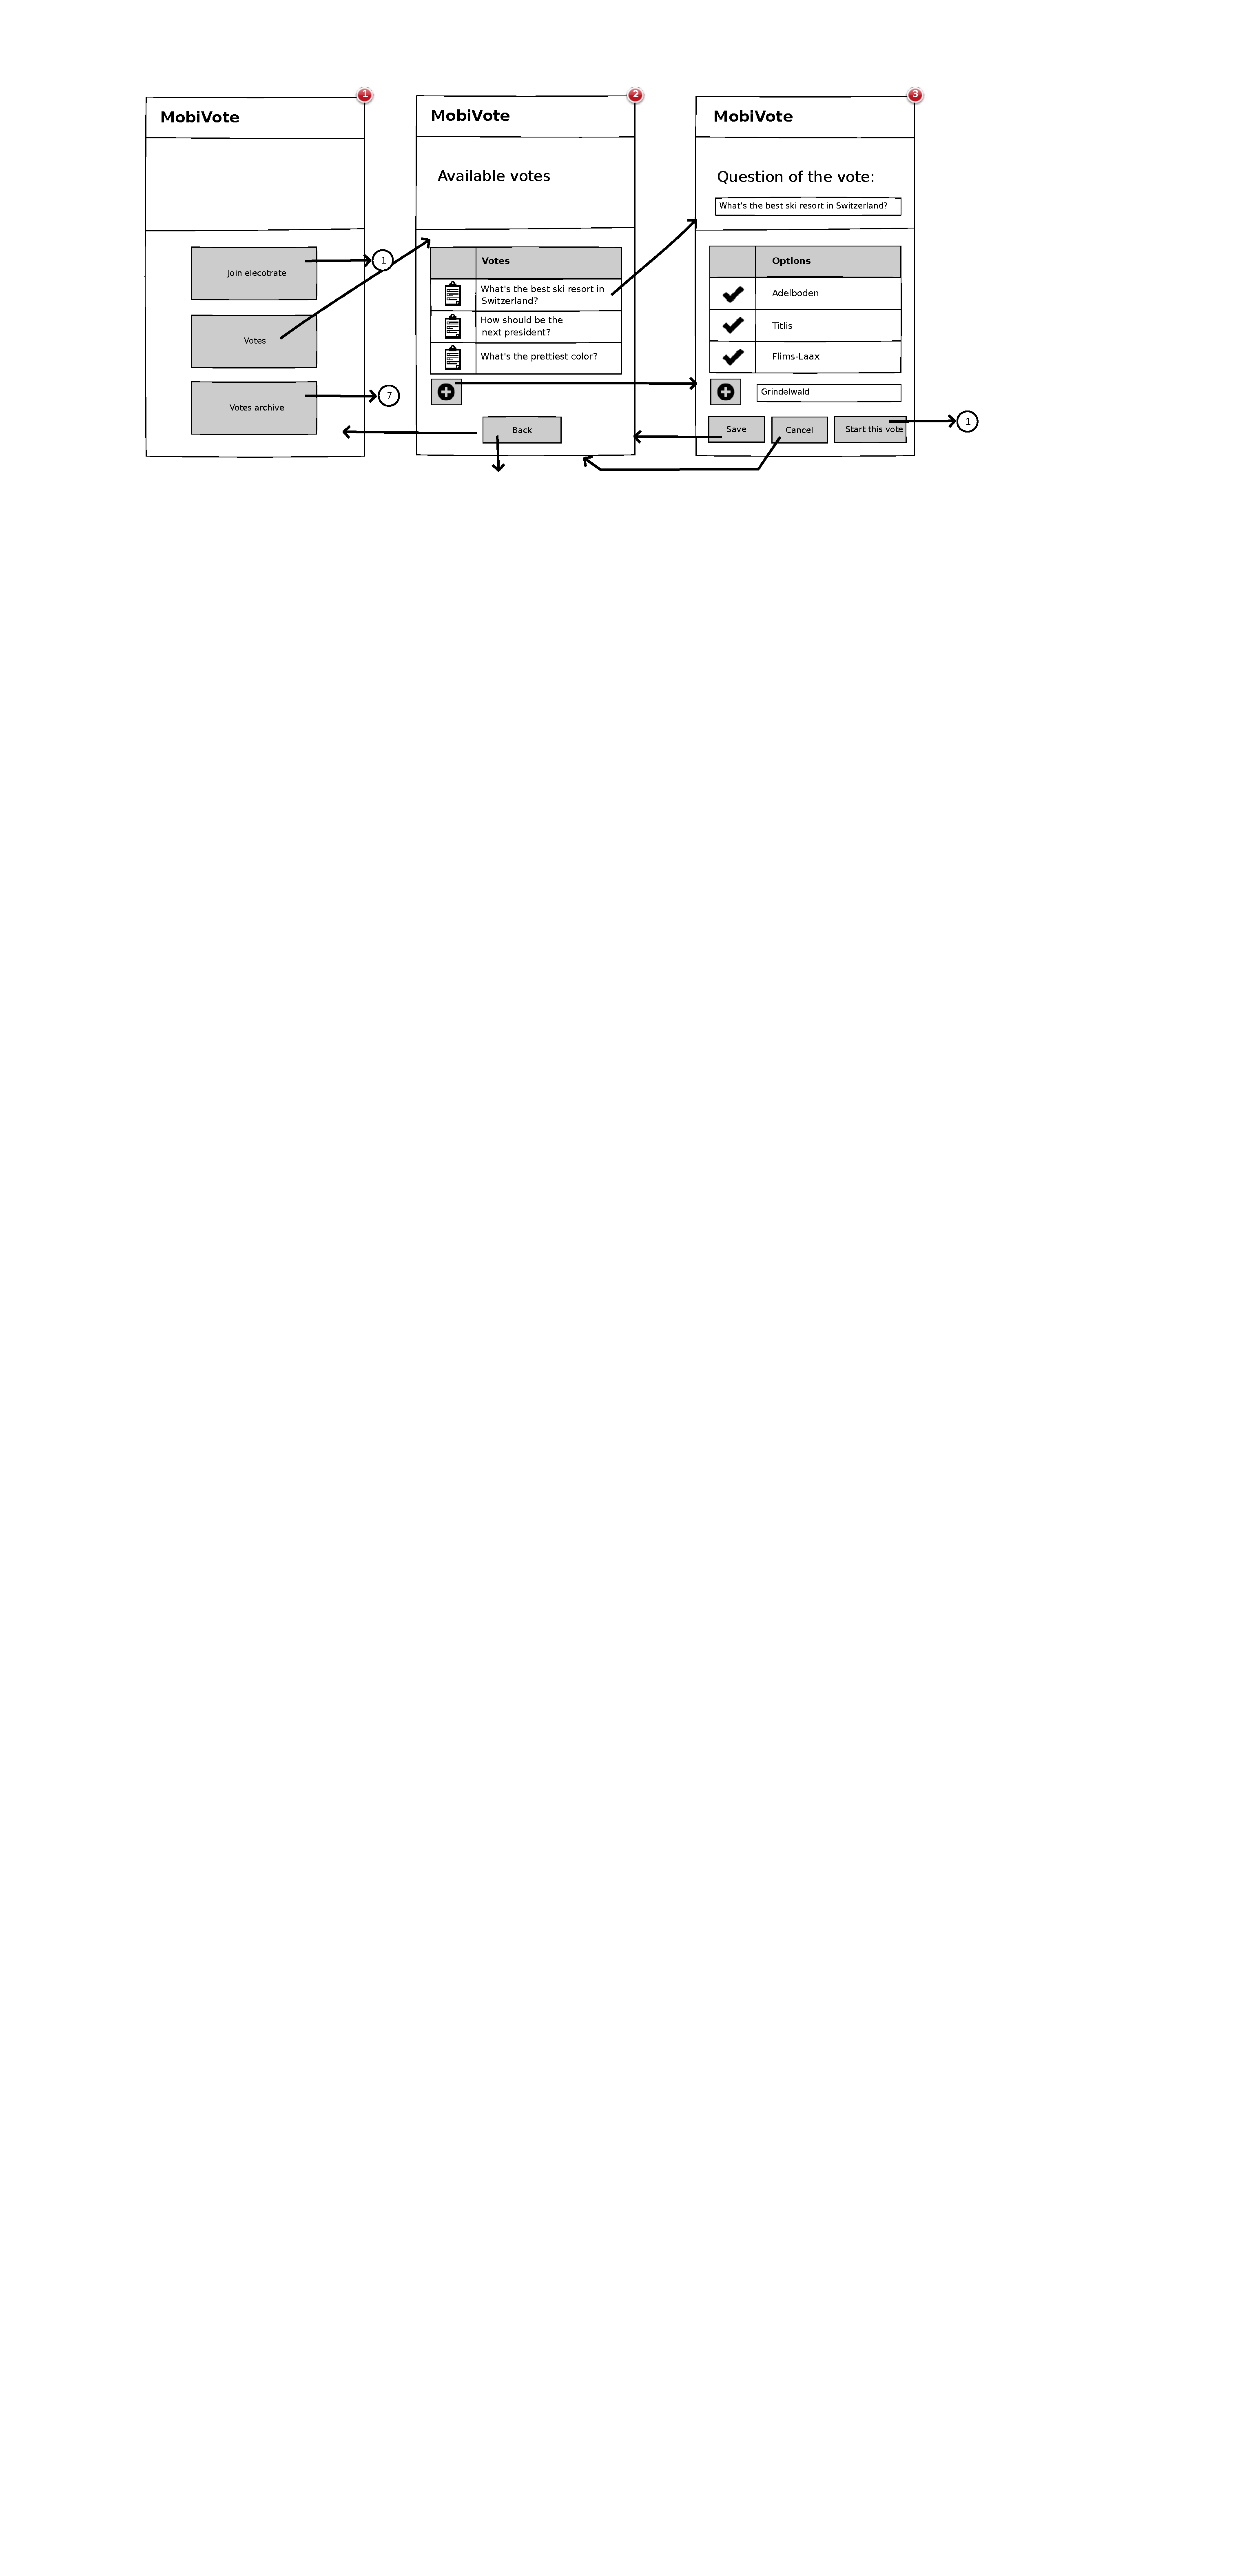
\includegraphics[height=.4\textheight]{img/vote_setup}
	\caption{Setup a vote}
	\label{fig:vote_setup}
\end{figure}

\paragraph{Network Setup.}
The next step after defining a vote is to define in which network environment
the voting session will take place. The first person to do so is the vote
administrator. He can choose a Wi-Fi network in which the network session will
be started. The information about the chosen network as well as the generated
session password has to be shared with the participants. To do so, the
administrator can either just read the information out loud, or share the
information using either a QR-code or write the information to a NFC token which
can be passed to all participants. Using this information, the participants can
join the network session with their devices. Before joining the session, each
participant (including the administrator) has to define an identification string
for themselves. The screen design of this phase is illustrated in
\Vref{fig:network_setup}.

\begin{figure}[htbp]
	\centering
	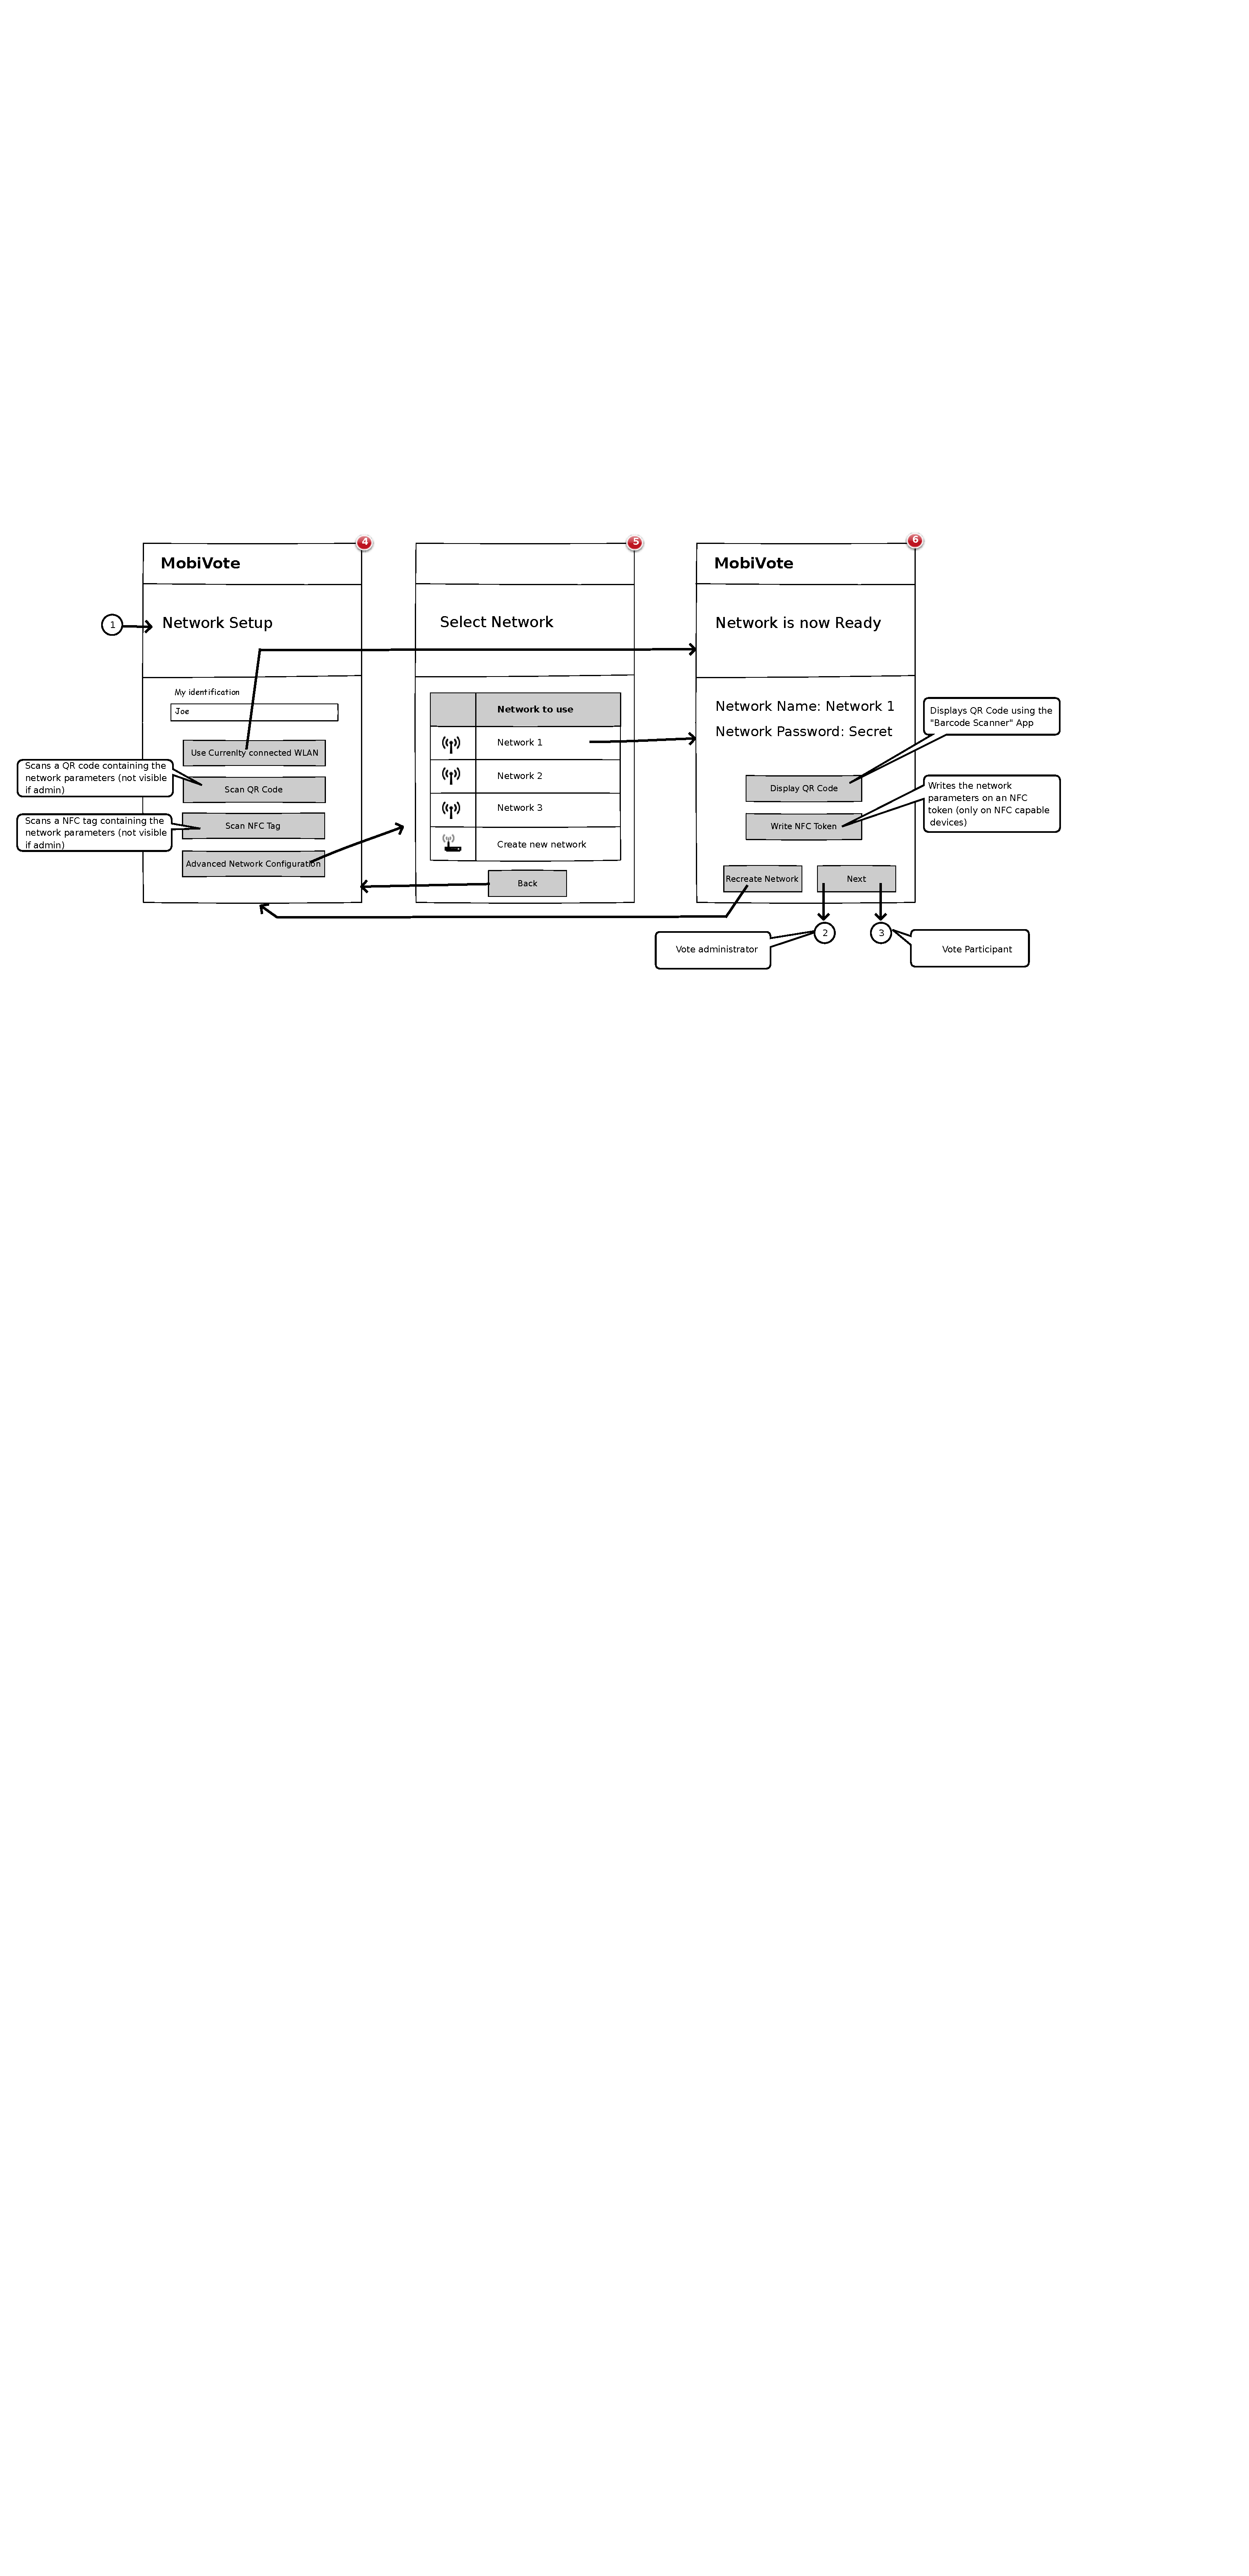
\includegraphics[height=.4\textheight]{img/network_setup}
	\caption{Network setup}
	\label{fig:network_setup}
\end{figure}


\paragraph{Defining the Electorate and Review of the Vote.}
After joining the network session, a list of all the session participants is
displayed. At this stage, the administrator can define the electorate, meaning
he can select the participants which are allowed to vote. This can be done by
clicking on the the checkboxes next to the participant's identification. The
participants can see who has been selected on their devices.

Once the administrator has defined the electorate, each participant has to
confirm that all the parameters of the vote (question, allowed options
and electorate) are correct. The vote can only be started by the administrator
if the whole electorate has agreed. If necessary, the administrator can go back and do changes on the vote parameters.

The screen design of this phase from the administrator's perspective is
illustrated in \Vref{fig:admin_review} and from the voter's perspective in
\Vref{fig:voter_review}.

\begin{figure}[htbp]
	\centering
	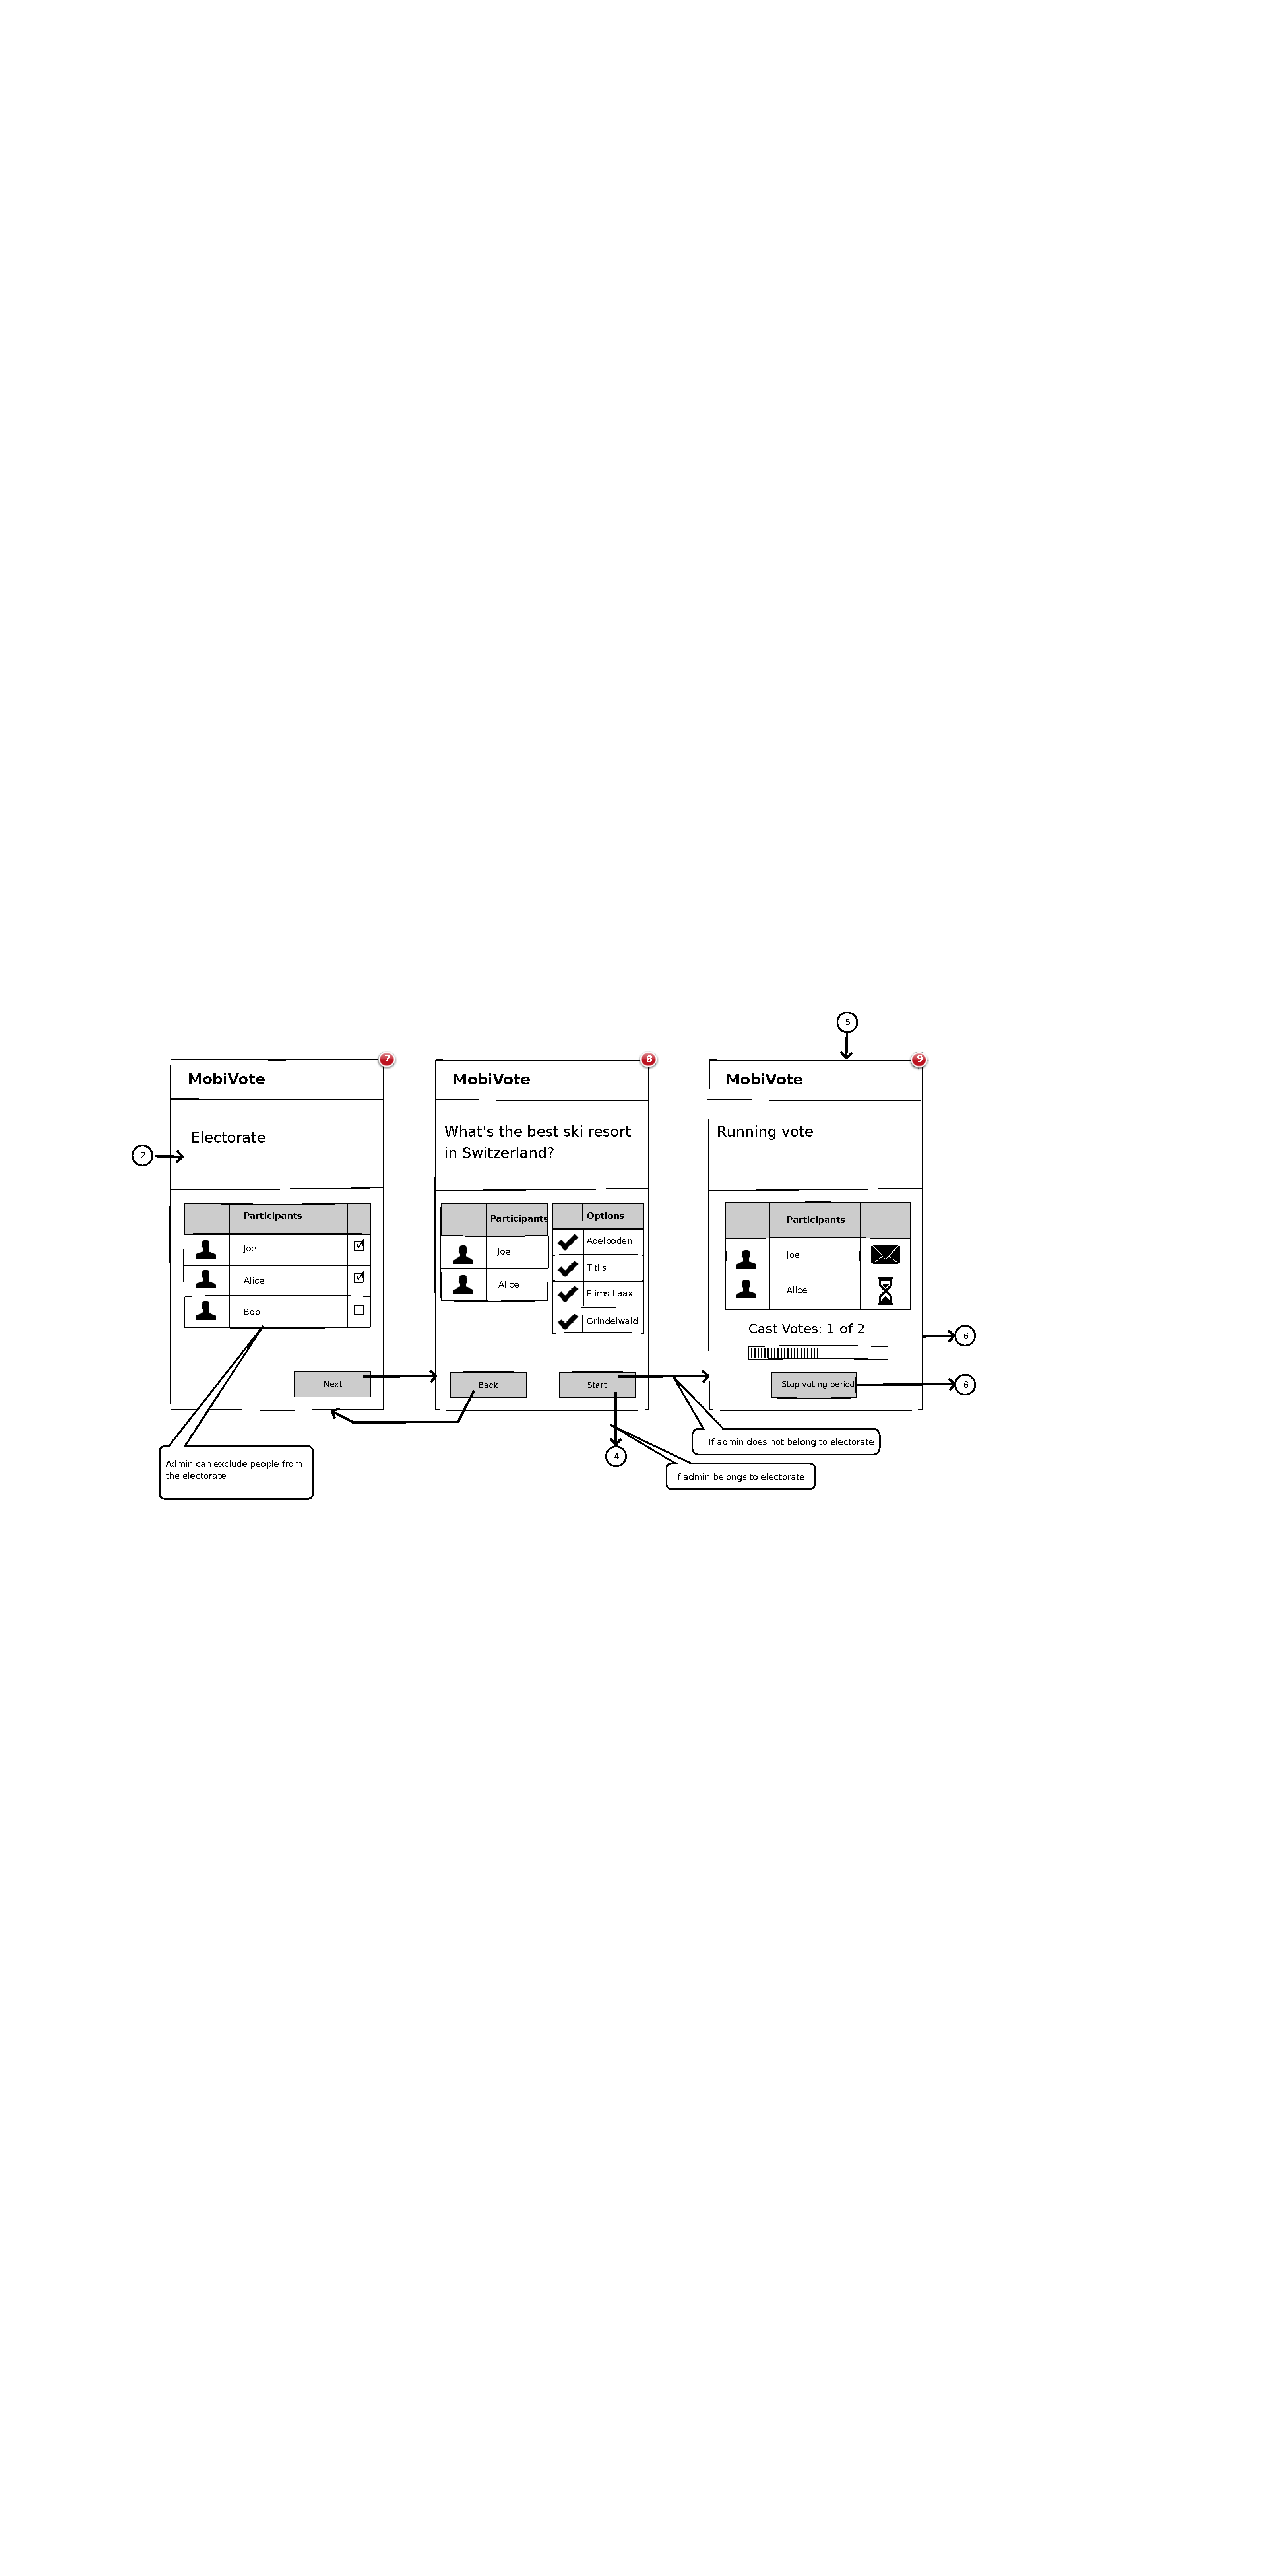
\includegraphics[height=.4\textheight]{img/admin_review}
	\caption{Administrator defining the electorate}
	\label{fig:admin_review}
\end{figure}

\begin{figure}[htbp]
	\centering
	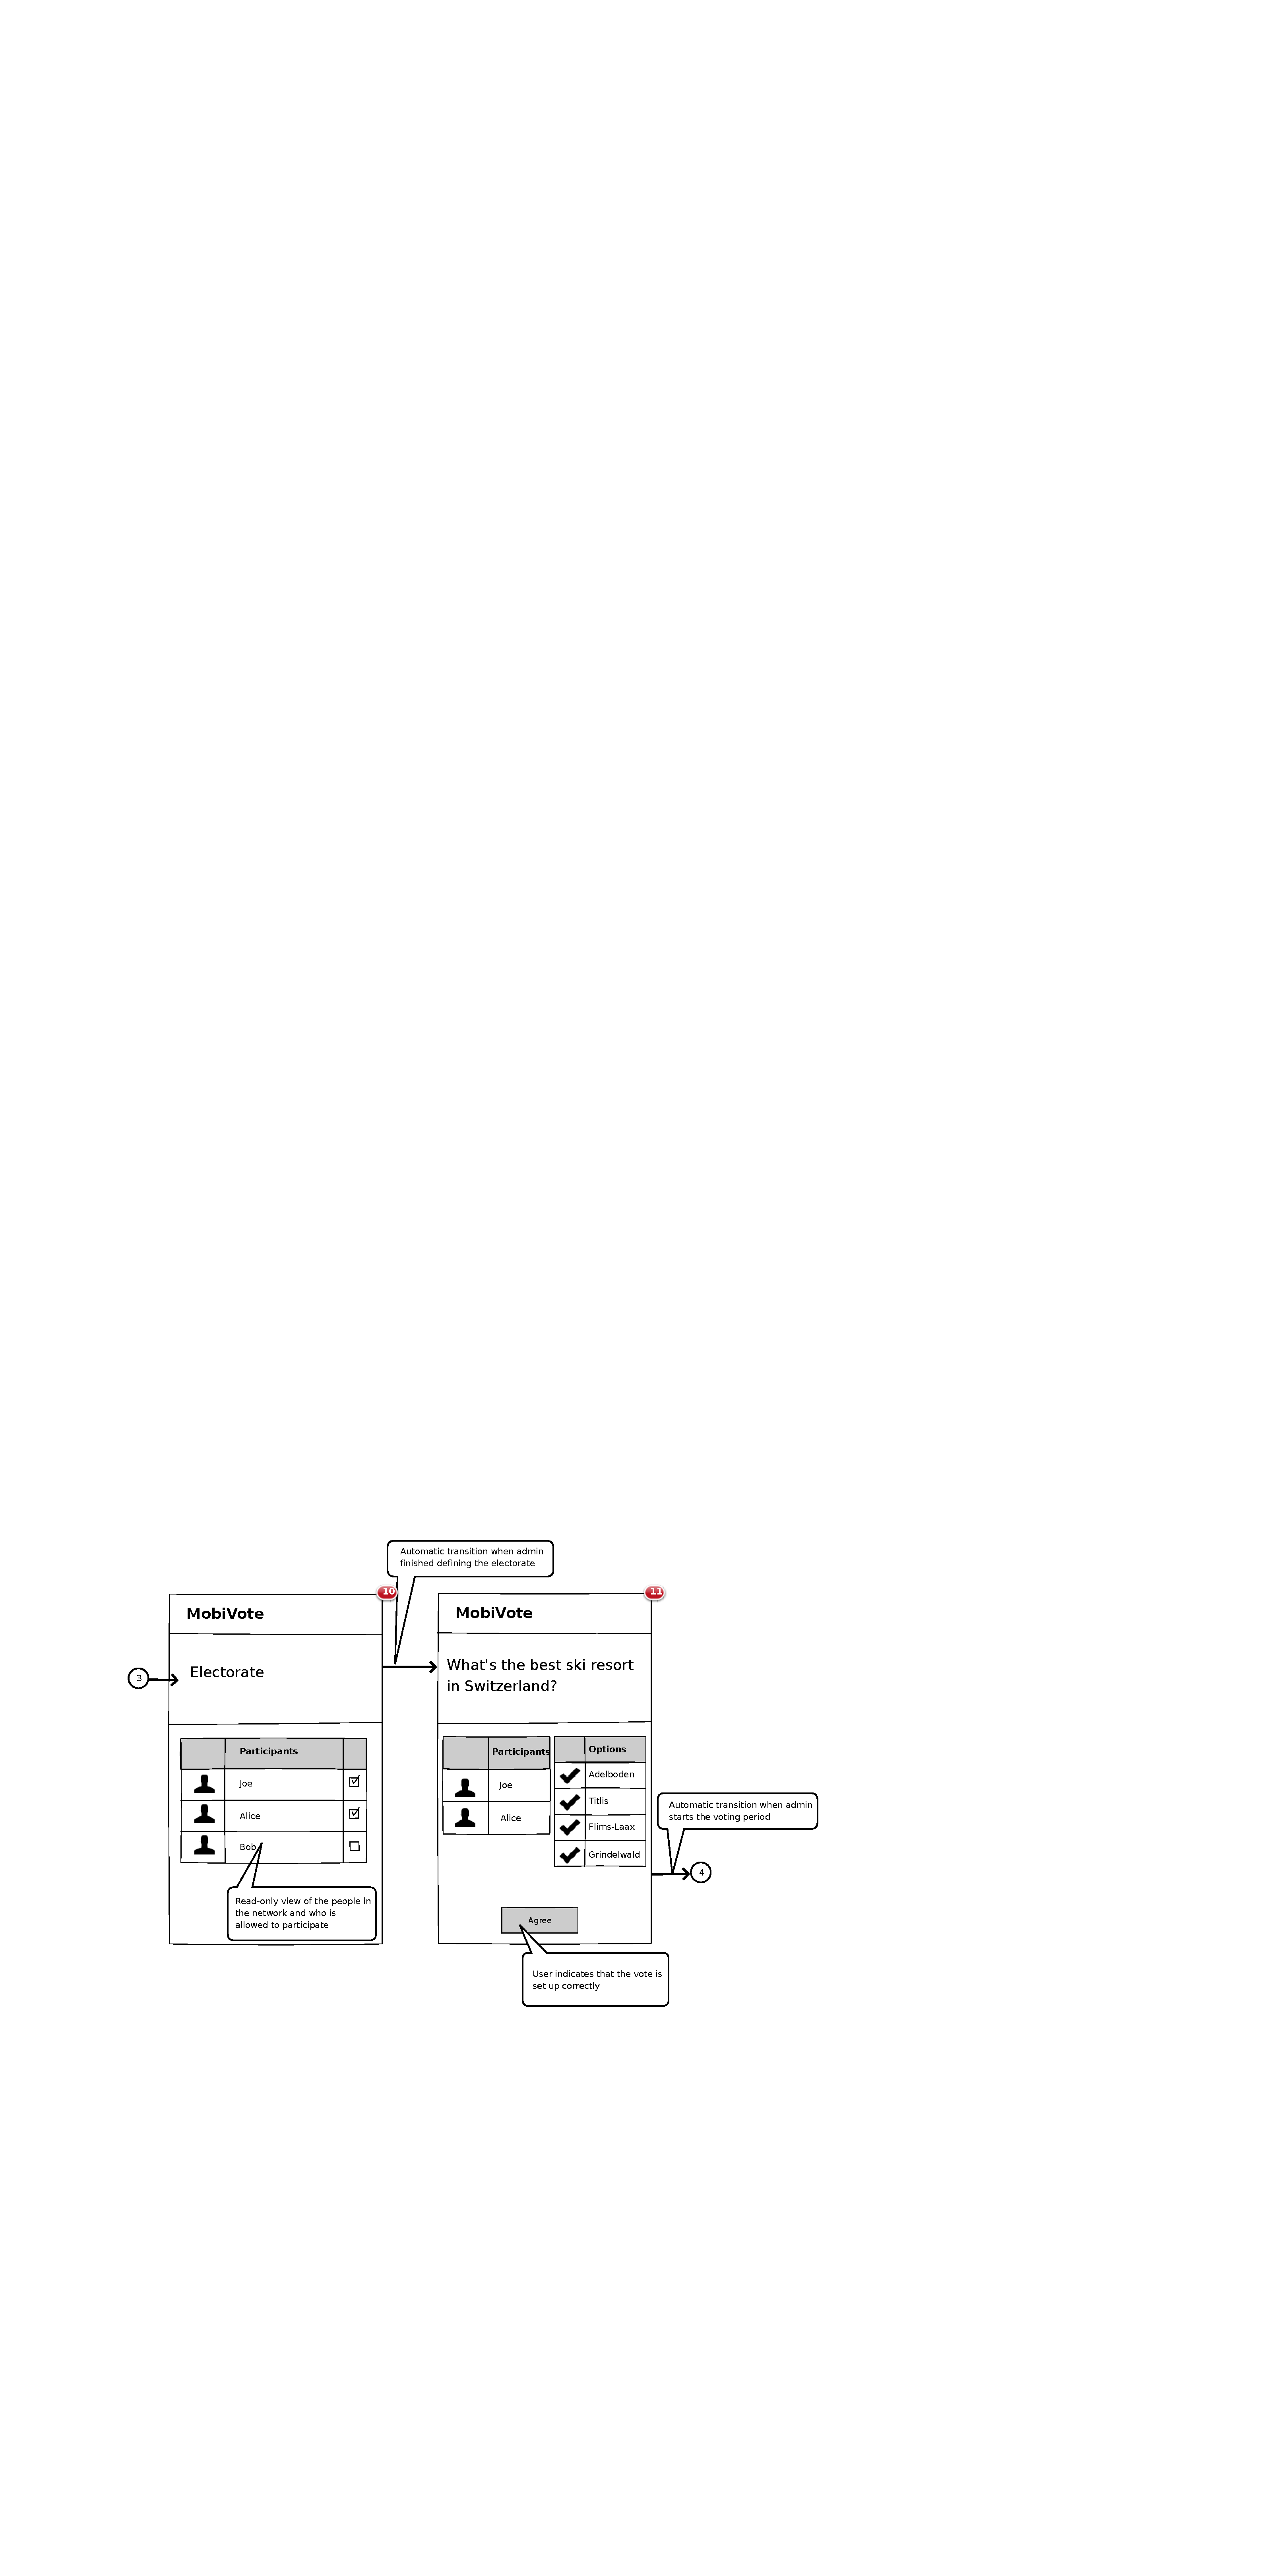
\includegraphics[height=.4\textheight]{img/voter_review}
	\caption{Review of the vote from voter's perspective}
	\label{fig:voter_review}
\end{figure}

\paragraph{Voting phase.}
Once the vote has passed the review, the vote itself can take place. Each
participant can choose an option and cast it. The screen transitions to a view
which shows the vote casting state of all the participants. The screen
design of this phase is illustrated in \Vref{fig:vote}.

\begin{figure}[htbp]
	\centering
	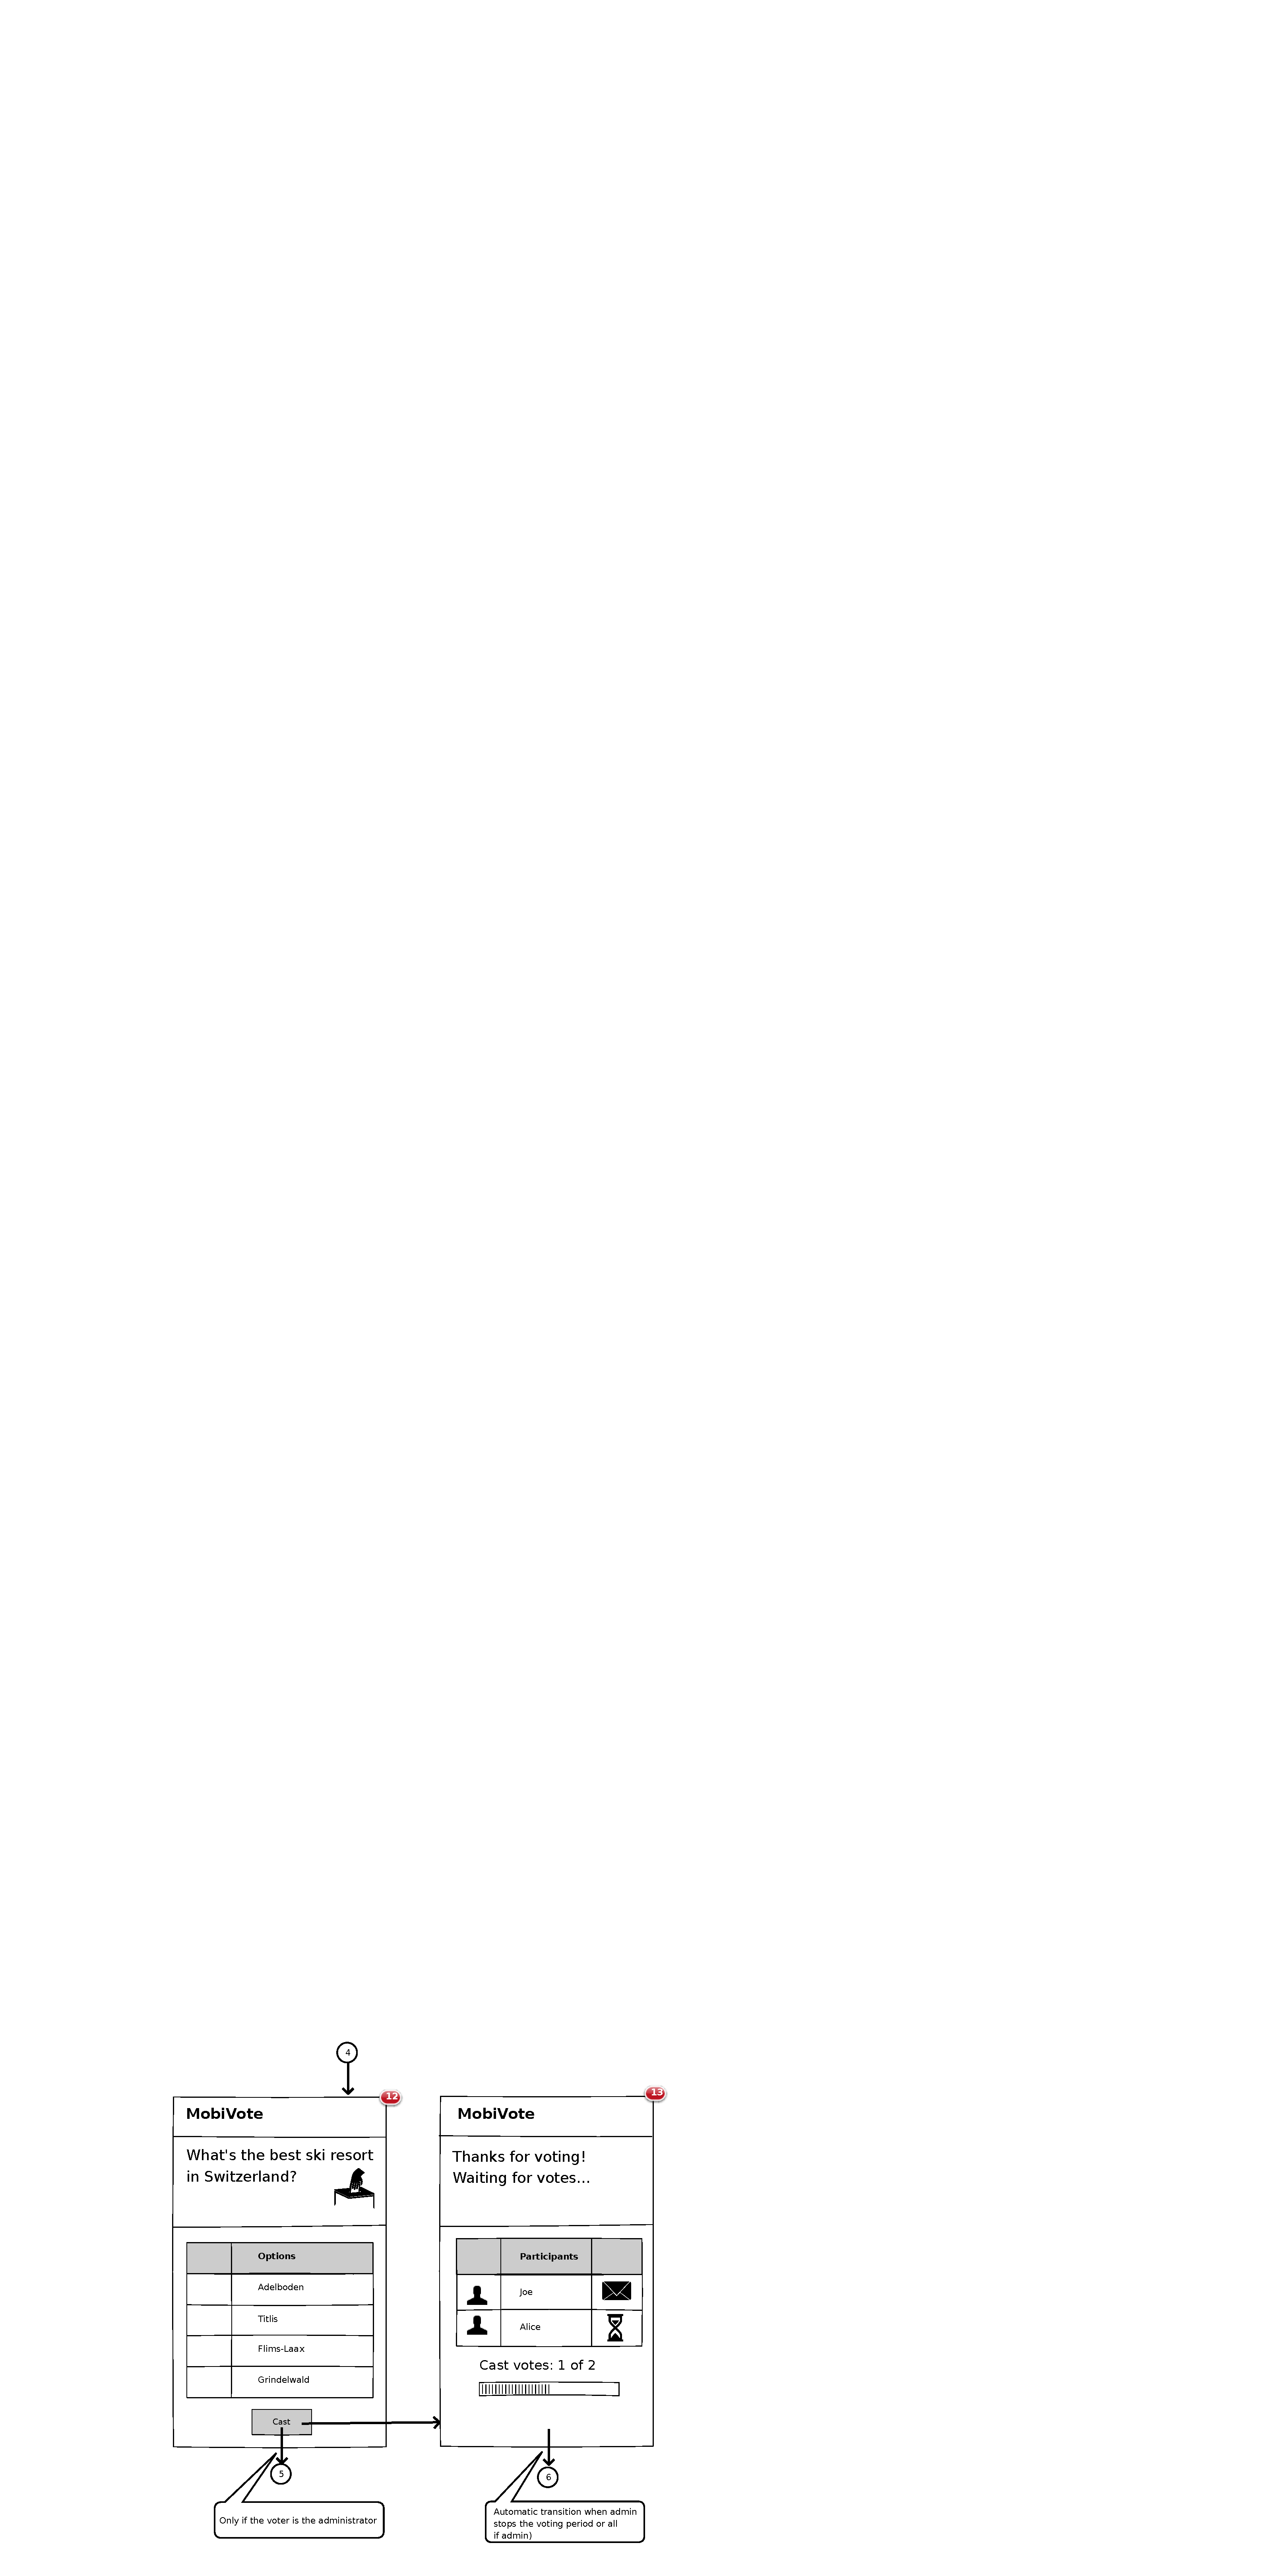
\includegraphics[height=.4\textheight]{img/vote}
	\caption{Vote casting}
	\label{fig:vote}
\end{figure}

\paragraph{Displaying the result.}
The vote is tallied as soon as the last vote has been cast, or if the
administrator has ended the voting phase. The result is displayed in the form of
a piechart and a tabular view. The result of the vote is saved on each devices
and can be revisited using the archive function in the main screen. The screen
design of this phase is illustrated in \Vref{fig:result}.

\begin{figure}[htbp]
	\centering
	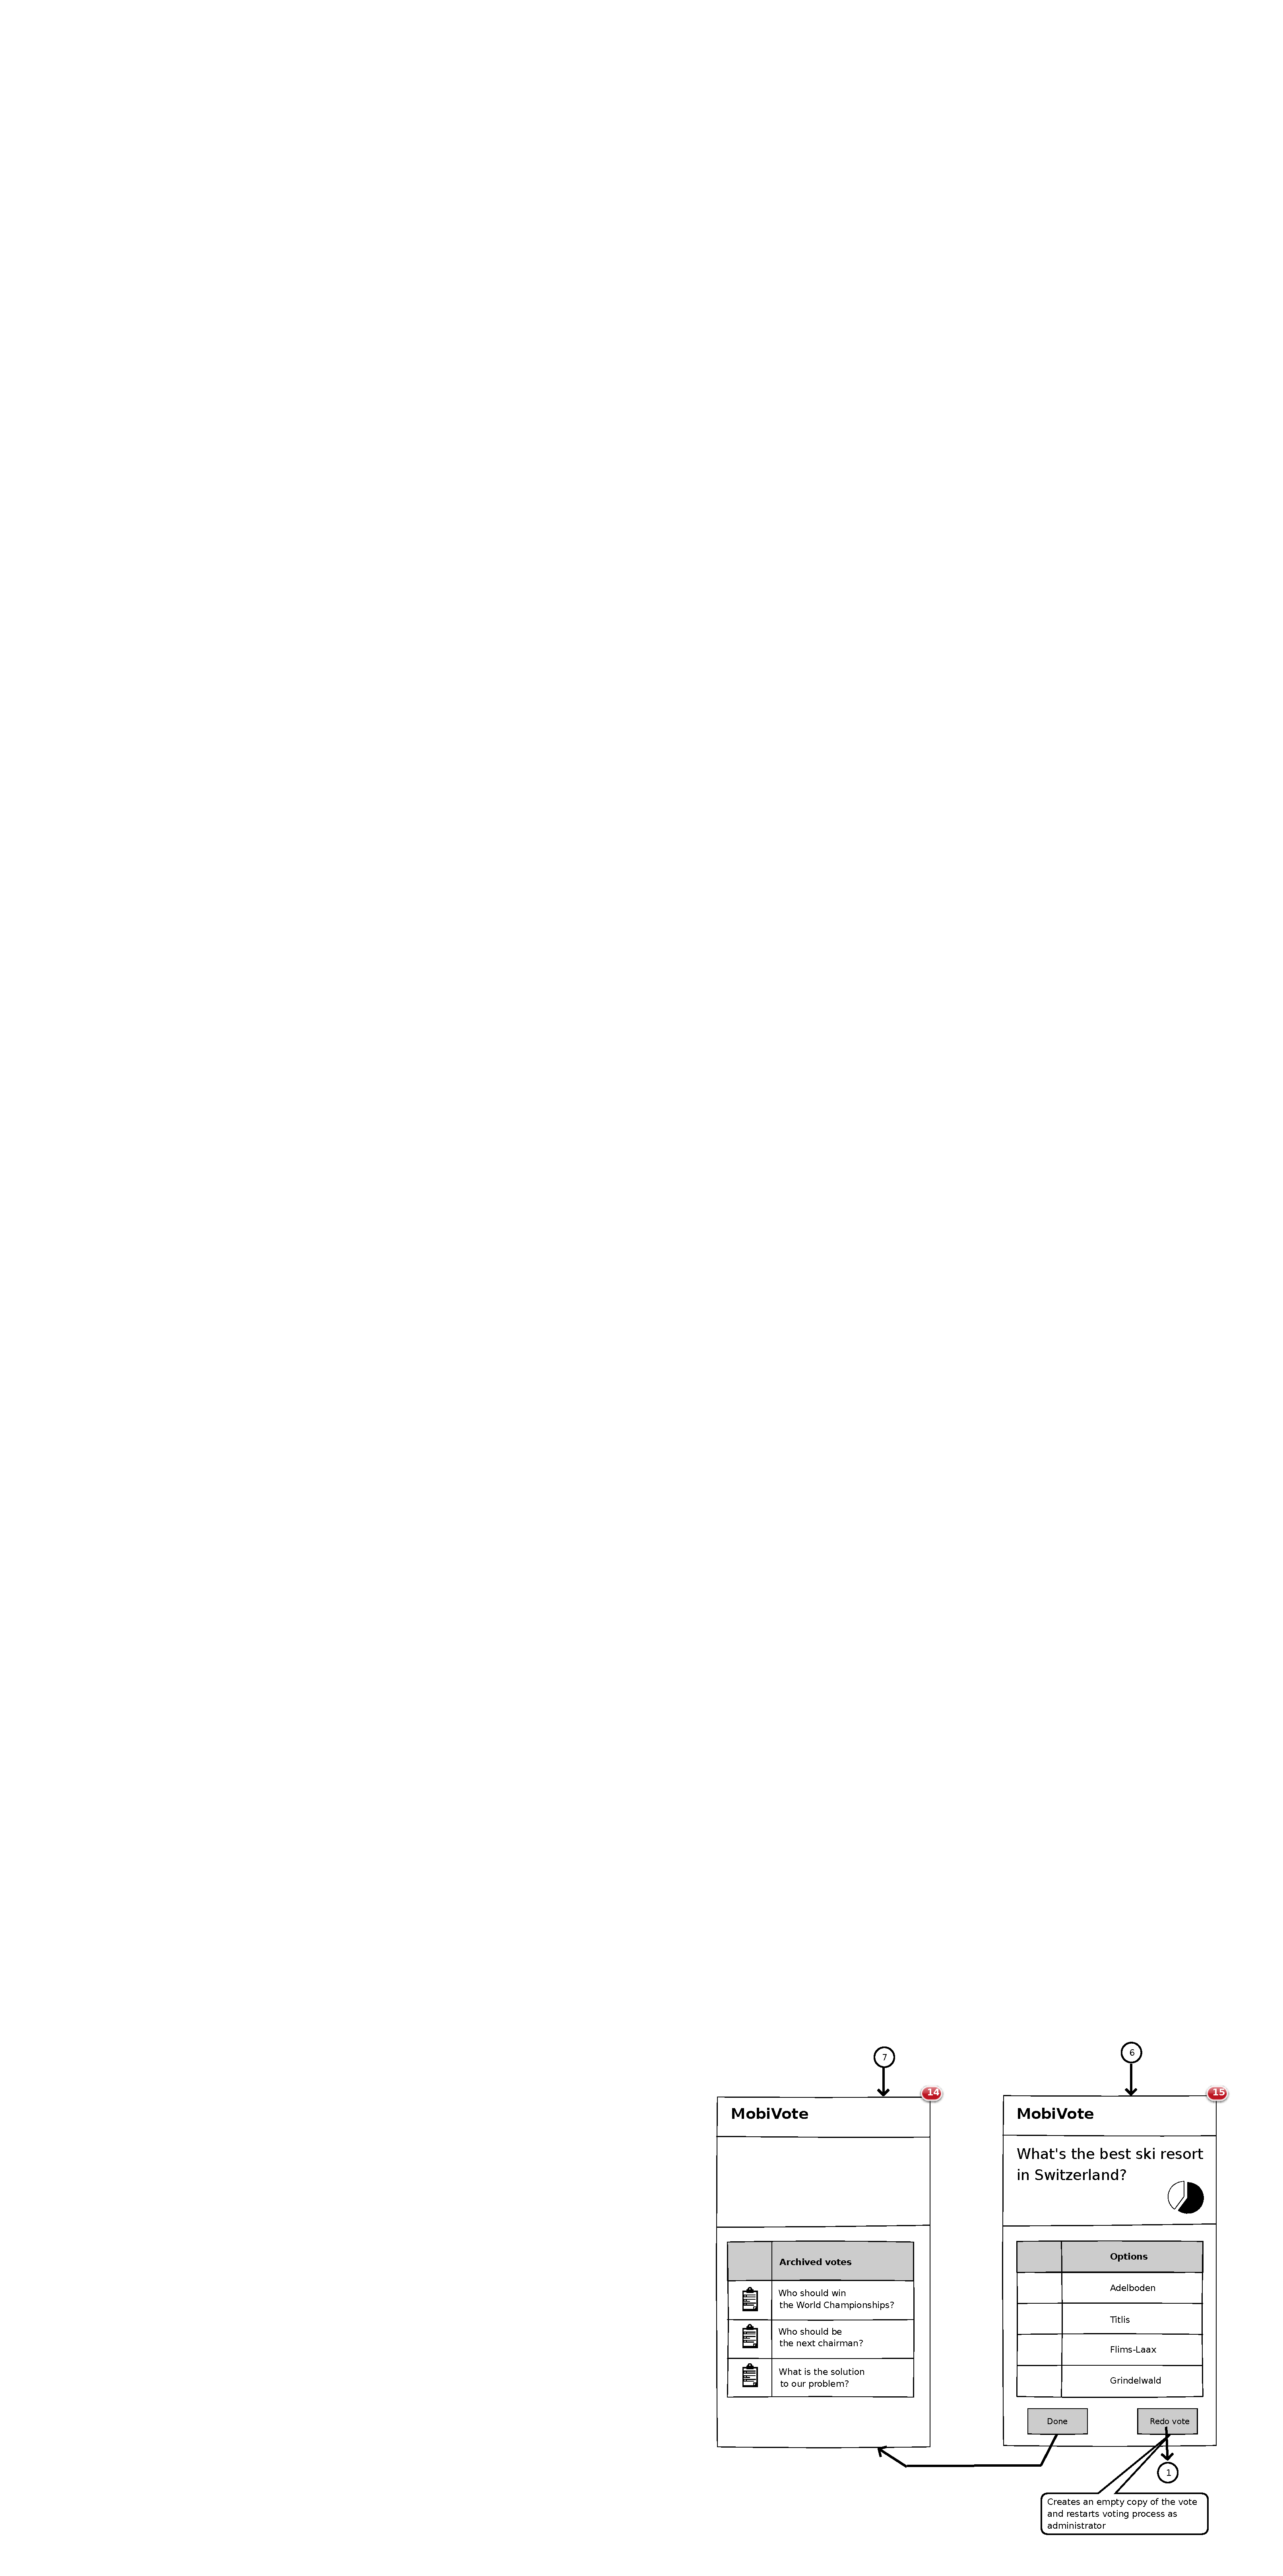
\includegraphics[height=.4\textheight]{img/result}
	\caption{Result of the vote}
	\label{fig:result}
\end{figure}


\section{Implementation}
\label{sec:implementation}
\todo{This chapter will be written in a later phase of the project}


\subsection{Used Technologies}
This Section outlines the frameworks which have been used for the implementation
of this project and how they are put together into an application.
\subsubsection{Android}
The Android\footnote{\url{http://developer.android.com/}} platform serves as the
foundation of the whole implementation. The Application has been built using existing building blocks such as Activities,
Services, Fragments, etc. Furthermore, there are existing guidelines and best
practices which have been employed whenever possible. 



\subsubsection{AllJoyn}
AllJoyn\footnote{\url{https://allseenalliance.org/}} is a library which allows
peer-to-peer communication between several devices. The library has been
released as opensource recently by the Qualcomm company. It is available for
multiple platforms, including Android. AllJoyn serves as a communication layer
which allows to exchange messages between devices such as smartphones and
tablets. One device acts as master and starts advertising a group to which other
devices can join. Once joined into the group, all the devices in the group can
exchange messages among each other. The communication can happen either in
broadcast (one to many) or unicast (one to one).

The original intention was to use InstaCircle \cite{ritter13a} as a
communication layer. It turned out that this type of completely decentralized
communication layer did not suit our needs and did not work as expected in some
network configurations. Compared to InstaCircle, AllJoyn bears the drawback that
the communication is orchestrated on the master device that initiates the group
communication. In exchange, the communication is reliable.

Some parts of InstaCircle were used, mainly the WLAN management and the logic
for transmiting the communication parameters could be adapted from the
InstaCircle implementation.

\subsubsection{ZXing}
ZXing\footnote{\url{https://code.google.com/p/zxing/}} (pronounced ``Zebra
Crossing'') is a Java library provided by Google which allows to deal with many
flavours of barcodes, including QR-codes which we are using in this
implementation. It provides the logic to encode information into a QR-code and
display it on the user interface of the application. It also provides the
functionality to use the camera of a smartphone/tablet as a scanner in order to
decode the QR-code which is being displayed on the screen of another device.

In this project, we are using this functionality for transmiting the parameters
of the group to other devices. These parameters include the SSID of the WLAN
that is being used, the encryption key of the conversation, as well as a group
identifier in case there are multiple conversations running in the same network.

\subsubsection{AChartEngine}
AChartEngine\footnote{\url{http://www.achartengine.org/}} is an opensource
library which can be used to draw all sorts of charts on Android devices. In
this project, we use this library in order to visualize the result on the
result screen using a pie chart.

\subsubsection{UniCrypt}
UniCrypt\footnote{\url{https://github.com/bfh-evg/unicrypt/}} is a cryptographic
library which provides mathematical and cryptographic primitives which are used
for implementing the e-voting protocol for this application. The version 2 of
UniCrypt is currently under active development. The use of this library in this
project also helped to improve UniCrypt itself. Since UniCrypt is developed at
the same institute, problems could be adressed and fixed right away. Since this
project is one of the first projects using UniCrypt, it also served as a test
bed for UniCrypt. For this project, some non existing extensions for UniCrypt
have been implemented. The result of this work is discussed in further detail in
\Vref{sec:enhancmentsunicrypt}.

Since UniCrypt is an essential cornerstone of this project, it is discussed in
further detail in \Vref{sec:unicrypt}.

\section{Graphical User Interface}
\label{sec:graphicaluserinterface}

The Android platform provides a powerful framework which allows to design rich
user interfaces specifically designed for mobile devices. The User interface was
built using these techniques.

\paragraph{Activities.}
Android Activities basically represent screens which allow the user to interact
with the application. An activity is represented as a Java class inheriting from
the Activity class. For each Activity there is a XML file which represents the
structure of the screen layout and which elements (buttons, icons, labels,
textfields, etc.) it contains. \Vref{tab:activities} outlines the activities and
the corresponding layouts which have been implemented for this application.

\begin{table}[htbp]
	\centering
	\begin{tabularx}{\textwidth}{llX}
		\toprule
		\textbf{Activity}			& \textbf{Layout}							& 	\textbf{Description}			\\
		\midrule
		CheckElectorateActivity 	& \texttt{activity\_check\_electorate.xml} 				&		\\
		CreateNetworkActivity		& \texttt{activity\_create\_network.xml}				&		\\
		DisplayResultActivity		& \texttt{activity\_display\_result.xml}				&		\\
		ElectorateActivity			& \texttt{activity\_electorate.xml}						&		\\
		ListTerminatedPollsActivity	& \texttt{activity\_list\_terminated\_polls.xml}		&		\\
		MainActivity				& \texttt{activity\_main.xml}							& 	 	\\
		NetworkConfigActivity		& \texttt{activity\_network\_config.xml}				&		\\
		NetworkInformationActivity	& \texttt{activity\_network\_information.xml}			&		\\
		PollActivity				& \texttt{activity\_poll.xml}							& 		\\
		PollDetailActivity			& \texttt{activity\_poll\_detail.xml}					&		\\
		ReviewPollAdminActivity		& \texttt{activity\_review\_poll.xml}					&		\\
		ReviewPollVoterActivity		& \texttt{activity\_review\_poll\_voter.xml}			&		\\
		VoteActivity				& \texttt{activity\_vote.xml}							&		\\
		WaitForVotesAdminActivity	& \texttt{activity\_admin\_wait\_for\_votes.xml}		&		\\
		WaitForVotesVoterActivity	& \texttt{activity\_wait\_for\_votes.xml}				&		\\
		
		\bottomrule
	\end{tabularx}
	\caption{Activities}
	\label{tab:activities}
\end{table}


\paragraph{Fragments.}
Fragments allow to reuse parts of a screen design in multiple activities. They
are also used to design complex dialog interfaces. Fragments are always embedded
into an activity or a dialog. Similar to activities,
fragments also have a corresponding layout which is stored
in a XML file. \Vref{tab:fragments} outlines the fragments and the corresponding
layouts which have been implemented for this application.

\begin{table}[htbp]
	\centering
	\begin{minipage}{\linewidth}
	\begin{tabularx}{\textwidth}{llX}
		\toprule
		\textbf{Fragment}						& \textbf{Layout}				& 	\textbf{Description}			\\
		\midrule
		ConnectNetworkDialogFragment			& \texttt{dialog\_join\_network.xml}			& 	\\
		HelpDialogFragment						& \texttt{dialog\_help.xml}						& 	\\
		IdentificationWlanKeyDialogFragment		& \texttt{dialog\_identification\_wlankey.xml}	&	\\
		NetworkDialogFragment					& \texttt{dialog\_network\_information.xml}		&	\\
		NetworkInformationFragment				& \texttt{fragment\_network\_information.xml}	&	\\
		NetworkListFragment						& \texttt{list\_item\_network.xml}\footnote{In
		\emph{ListFragments} the layout for each row is applied} 								&	\\
		NetworkOptionsFragment					& \texttt{fragment\_network\_options.xml}		& 	\\
		NFCFragment								& \texttt{fragment\_nfc.xml}					&	\\
		PollReviewFragment						& \texttt{fragment\_poll\_review.xml}			&	\\
		ResultChartDialogFragment				& \texttt{dialog\_chart.xml}					&	\\
		ResultChartFragment						& \texttt{fragment\_result\_chart.xml}			&	\\
		WaitForVotesFragment					& \texttt{fragment\_wait\_for\_votes.xml}		&	\\
		\bottomrule
	\end{tabularx}
	\end{minipage}
	\caption{Fragments}
	\label{tab:fragments}
\end{table}

\section{Bootstrapping of Group Communication}
\label{sec:bootstraping}
A challenge of the 


\section{Messaging}
\label{sec:messaging}

\section{Datastructures}
\label{sec:datastructures}

\section{Voting Protocol}
\label{sec:votingprotocol}


\section{UniCrypt Extensions}
\label{sec:enhancmentsunicrypt}
The CGS97 protocol contains a few building blocks which were not part of the
UniCrypt library by the time this project started. Part of the goals of this
project was to enhance UniCrypt so that the logic could be used in the
implementation of this application and make it also reusable in further upcoming
projects. In the following we describe how this implementation has been done.

\subsection{Shamir Secret Sharing Scheme}
In 1979, Adi Shamir proposed a scheme \cite{Shamir79} on how a secret can be
split into several independent pieces which can be distributed among several
authorities. It is not possible to recover the secret unless a sufficient amout
of these authorities collaborate in order to recover the secret. Further details
regarding this scheme can be found in \Vref{sec:secretsharing}.

\paragraph{Implementation.} The implementation has been embedded into the
existing UniCrypt structure.
The class in which the implementation has been done is the following:

\texttt{ch.bfh.unicrypt.crypto.schemes.sharing.classes.ShamirSecretSharingScheme}
\\
\\
The instanciation of this scheme requires three parameters:
\begin{itemize}
  \item An algebraic field of the type \\
  \texttt{ch.bfh.unicrypt.math.algebra.dualistic.classes.ZModPrime}. The secret
  which should be shared later on has to be an element of this field.
  \item The number of shares which should be produced
  \item A threshold value which defines how many shares must be reunited in
  order to recover the secret
\end{itemize}

A secret can be shared using the method \texttt{share()}, which takes
a message as an argument. The message must be an element of the field which has
been specified during the initialisation of the scheme. The method returns an
array of value pairs. Each pair represents a share.

The secret can be recovered using the method \texttt{recover()}, which takes an
array of value pairs as an argument. The array must at least contain as many
value pairs as specified with the threshold value during instantiation. The
method returns a single element which represents the recovered secret.

\paragraph{Testing.}
UniCrypt components are tested using the JUnit framework. A JUnit Test for the
Shamir Secret Sharing scheme has been implemented in order to check the correct
functionality after each change that is done in the UniCrypt library. The
following testclass has been implemented:

\texttt{ch.bfh.unicrypt.crypto.schemes.sharing.ShamirSecretSharingSchemeTest}

\subsection{ElGamal Proof of Validity}
A proof of validity is required if a party wants to prove that an ElGamal
ciphertext is the encryption of element of a set of possible plaintexts without
revealing which one it is. \Vref{sec:proofofvalidity} covers this topic in
further detail.

The implementation of the this proof has been done in a very early stage of this
project, according to the architecture of UniCrypt 1. In the meantime, UniCrypt
has been completely reengineered. The validity proof has been reimplemented
independently of this project in order to fit into the new architecture. Since
this project is based on UniCrypt 2, the project makes use of the reimplemented
version of the ElGamal proof of validity.


\chapter{Discussion}
\label{cha:discussion}
\todo{This chapter will be written in a later phase of the project}

\chapter{Conclusion}
\label{cha:conclusion}
\todo{This chapter will be written in a later phase of the project}

\printbibliography

\appendix

\chapter{Planning}

\begin{sidewaysfigure}[ph]
\noindent\resizebox{\textwidth}{!}{
	\begin{tikzpicture}[x=.5cm, y=1cm]
	\begin{ganttchart}
	[vgrid, hgrid,
	group/.style={draw=black, fill=black!50}, y unit chart=0.8cm]{26}
	\gantttitle{\textbf{Planning Master Thesis (part 1)}}{26} \\
	\gantttitlelist{8,...,33}{1} \\
	\ganttmilestone{Kickoff}{0.5} \\
	\ganttgroup{Writing of Project Proposal}{1}{6} \\
	\ganttgroup{Secret Sharing scheme}{6}{10} \\
	\ganttbar{Analyzing the possibilities of threshold secret sharing}{6}{8} \\
	\ganttbar{Implementing secret sharing into UniCrypt}{7}{10} \\
	\ganttbar{Testing the secret sharing scheme}{9}{10} \\
	\ganttgroup{Proof of Validity}{11}{13} \\
	\ganttbar{Implementing proof of validity into UniCrypt}{11}{12} \\
	\ganttbar{Testing of the proof of validity implementation}{12}{13} \\
	\ganttgroup{Evaluation of UniCrypt on Android}{14}{15} \\
	\ganttbar{Testing out Example code on Android}{14}{14} \\
	\ganttbar{Integration of code into Android project}{15}{15} \\
	\ganttmilestone{Building blocks ready}{15.5} \\
	\ganttgroup{Implementation of e-voting Application of Android}{20}{26} \\
	\ganttbar{Design of storyboard}{20}{24}\\
	\ganttbar{Implementation of the User Interface}{23}{26}\\
	\ganttbar[bar height=0.0, bar/.style={draw=none}]{Implementation of the
	e-voting logic}{0}{0}\\
	\ganttgroup[group height=0.0, group/.style={draw=none}]{Testing}{0}{0} \\
	\ganttgroup{Documentation / Report}{1}{8} \\
	\ganttmilestone[milestone height=0.0, milestone/.style={draw=none}]{Hand in}{0}	
	\end{ganttchart}
	\end{tikzpicture}
}
\caption{Planning part 1}
\label{fig:planningpart1}
\end{sidewaysfigure}
	

\begin{sidewaysfigure}[ph]
\noindent\resizebox{\textwidth}{!}{
	\begin{tikzpicture}[x=.5cm, y=1cm]
	\begin{ganttchart}
	[vgrid, hgrid,
	group/.style={draw=black, fill=black!50}, y unit chart=0.8cm]{26}
	\gantttitle{\textbf{Planning Master Thesis (part 2)}}{26} \\
	\gantttitlelist{34,35,36,37,38,39,40,41,42,43,44,45,46,47,48,49,50,51,52,1,2,3,4,5,6,7}{1}
	\\
	\ganttmilestone[milestone height=0.0,
	milestone/.style={draw=none}]{Kickoff}{0.5} \\
	\ganttgroup[group height=0.0, group/.style={draw=none}]{Writing of Project
	Proposal}{}{} \\
	\ganttgroup[group height=0.0, group/.style={draw=none}]{Secret Sharing
	scheme}{0}{0} \\
	\ganttbar[bar height=0.0, bar/.style={draw=none}]{Analyzing the possibilities
	of threshold secret sharing}{0}{0} \\
	\ganttbar[bar height=0.0, bar/.style={draw=none}]{Implementing secret sharing
	into UniCrypt}{0}{0}
	\\
	\ganttbar[bar height=0.0, bar/.style={draw=none}]{Testing the secret sharing
	scheme}{0}{0} \\
	\ganttgroup[group height=0.0, group/.style={draw=none}]{Proof of
	Validity}{0}{0} \\
	\ganttbar[bar height=0.0, bar/.style={draw=none}]{Implementing proof of
	validity into UniCrypt}{0}{0} \\
	\ganttbar[bar height=0.0, bar/.style={draw=none}]{Testing of the proof of
	validity implementation}{0}{0} \\
	\ganttgroup[group height=0.0, group/.style={draw=none}]{Evaluation of UniCrypt
	on Android}{0}{0} \\
	\ganttbar[bar height=0.0, bar/.style={draw=none}]{Testing out Example code on
	Android}{0}{0} \\
	\ganttbar[bar height=0.0, bar/.style={draw=none}]{Integration of code into
	Android project}{0}{0} \\
	\ganttmilestone[milestone height=0.0,
	milestone/.style={draw=none}]{Building blocks ready}{0.5} \\
	\ganttgroup{Implementation of
	e-voting Application of Android}{1}{13} \\
	\ganttbar[bar height=0.0, bar/.style={draw=none}]{Design of
	storyboard}{0}{0}\\
	\ganttbar[bar height=0.0, bar/.style={draw=none}]{Implementation of the User
	Interface}{0}{0}\\
	\ganttbar{Implementation of the e-voting logic}{1}{13}\\
	\ganttgroup{Testing}{7}{19} \\
	\ganttgroup{Documentation / Report}{14}{24.5} \\
	\ganttmilestone{Hand in}{24.5}
	\end{ganttchart}
	\end{tikzpicture}
}
\caption{Planning part 2}
\label{fig:planningpart2}
\end{sidewaysfigure}

\chapter{User Handbook}
This chapter describes how the MobiVote Application can be used in practice.

\section{Requirements}
In order to run a vote using MobiVote, all the participants need to be in
posession of a mobile device such as a smartphone or a tablet computer running
at least Android 4.0 (Ice Cream Sandwich). All the devices also need to be WLAN
capable and the WLAN adapter has to be activated. Currently is not possible to
use mobile devices of other flavour as Apple iPhones or devices running Windows
mobile.

\section{Installation}
The MobiVote application is available as an APK file which can be installed on
Android devices. In order to install the APK file, the file needs to be
transfered the devices. The easiest way is to connect the Device to a computer
using the USB cable and copy the APK file to the device. Using a filemanager on
the mobile device, locate the APK file in your filesystem and install it by
clicking on it. For this to work, the option
Settings $\rightarrow$ Security $\rightarrow$ Unknown Sources
must be enabled. 



\listoftodos

\end{document}
